%! Author = Runge
%! Date = 29-12-2023

% Preamble
\documentclass[english,a4paper,compsoc,journal]{IEEEtran}
\overfullrule=10pt
\frenchspacing

% Packages
%! Author = Runge
%! Date = 29-12-2023

\title{Symbolic Parameter Estimation of Continuous-Time Markov Chains}

\author{
\IEEEauthorblockN{Lars Emanuel Hansen}
\IEEEauthorblockA{\textit{dept. of Computer Science} \\
\textit{AAU}\\
Aalborg, Denmark \\
leha20@student.aau.dk}
\and
\IEEEauthorblockN{Daniel Runge Petersen}
\IEEEauthorblockA{\textit{dept. of Computer Science} \\
\textit{AAU}\\
Aalborg, Denmark \\
dpet20@student.aau.dk}\\
\and
\IEEEauthorblockN{Sebastian Aaholm}
\IEEEauthorblockA{\textit{dept. of Computer Science} \\
\textit{AAU}\\
Aalborg, Denmark \\
saahol20@student.aau.dk}
}
%! Author = Runge
%! Date = 29-12-2023

% Packages
\RequirePackage{setup/clrscode4e}
\usepackage{amsmath}
\usepackage{amsthm}
\usepackage{amssymb}
\usepackage{amsbsy}
\usepackage{mathrsfs}
\usepackage{dsfont}
\usepackage{bbold}
\usepackage{booktabs}
\usepackage{tikz}
\usepackage{bbm}
\usetikzlibrary{positioning}
\usetikzlibrary{calc}

\tikzset{%
  zeroarrow/.style = {-stealth,dashed},
  onearrow/.style = {-stealth,solid},
  c/.style = {circle,draw,solid,minimum width=2em,
        minimum height=2em},
  t/.style = {rectangle,draw,solid,minimum width=2em,
        minimum height=2em}
}

% Packages with options set
\usepackage[hidelinks]{hyperref}
\usepackage[textsize=small,obeyDraft]{todonotes}
\usepackage[newfloat]{minted}
\usepackage[backend=biber,
    bibencoding=utf8,
    maxbibnames=20,
    style=ieee,
    citestyle=numeric-comp,
    url=false
]{biblatex}
\usepackage[acronym]{glossaries}

% Package setup
\setlength{\marginparwidth}{2cm} % todonotes width
\setminted{linenos, autogobble, breaklines, fontsize=\footnotesize, style=friendly, xleftmargin=1em, numbersep=5pt}
\addbibresource{bib/main.bib}

% Other setup and options
\newtheorem{theorem}{Theorem}
\newtheorem{definition}{Definition}
\newfloat{algorithm}{htb!}{lop}
\floatname{algorithm}{Algorithm}
\newcommand{\algorithmautorefname}{Algorithm}
\makeatletter
\newcommand*\bigcdot{\mathpalette\bigcdot@{.5}}
\newcommand*\bigcdot@[2]{\mathbin{\vcenter{\hbox{\scalebox{#2}{$\m@th#1\bullet$}}}}}
\makeatother
\makeglossaries


%! Author = Runge
%! Date = 29-12-2023

\newacronym{aau}{AAU}{Aalborg University}

% Document
\begin{document}
    %! Author = Runge
%! Date = 29-12-2023
\IEEEtitleabstractindextext{%
    \begin{abstract}
        This is a placeholder abstract.
        The whole template is used in semester projects at \gls{aau}.
    \end{abstract}
    \begin{IEEEkeywords}
        Formal Verification, Parameter Estimation, Decision Diagram
    \end{IEEEkeywords}
}

    \maketitle
    \IEEEdisplaynontitleabstractindextext

    \section{Introduction}\label{sec:introduction}
%This paper is about improving the runtime of Jajapy - a tool for estimating parameters in parametric models~\cite{goossens1993}.
%Introduce Markov models
Markov models are a class of probabilistic models that are used to describe the evolution of a system over time.
A Markov model has the Markov property, which states that the future behavior of the system depends only on its current state and not on its past history~\cite{markov1962theory}.
This property simplifies analysis by focusing only on the present state, making Markov models especially useful for systems where memory-less behavior is a reasonable assumption.

Markov models are widely used in various fields, such as biology, finance, and computer science, to model systems that exhibit stochastic behavior~\cite{covid19_prism,ciocchetta2009bio, mamon2007hidden,lazowska1984quantitative}.
As such, their analysis has a wide range of applications.

An example of a Markov model, is a simple weather model, if today is sunny, there might be an 80\% chance of sun tomorrow and a 20\% chance of rain.
Similarly, if today is rainy, there might be a 70\% chance of rain tomorrow and a 30\% chance of sun.

%Model checking
Model checking is a technique used to verify the correctness of Markov models by comparing the predictions of the model with observed data.
Model checking is widely used in the verification of Markov models, where the model is analyzed to check if it satisfies certain properties~\cite{clarke1997model}.
It ensures reliability and correctness in critical systems, from traffic controls to industrial automation and communication protocols~\cite{clarke1997model}.
It is also used to check if the model satisfies certain properties, such as reachability, can we reach a desired state and safety properties, can we avoid going a specific sequence of states.

A real world example of model checking is the verification of a traffic light system, where the model is analyzed to check if the traffic lights are working correctly.
For reachability, we can ask: \textit{can a traffic light system always cycle back to green after being red?}.
For safety properties we can ask, \textit{can a traffic light system avoid having both lights green at the same time?}.

There exists several tools for model checking, such as PRISM~\cite{kwiatkowska2011prism} and Storm~\cite{hensel2021probabilistic}, which are widely used in the verification of Markov models.
These tools use symbolic representations to represent the model and perform the operations required for model checking.
The limitation of these tools is that they do not support parameter estimation, which makes them unsuitable for learning the parameters of the model from data.

Parameter estimation is a crucial step in the analysis of Markov models, as the analysis of the model depends on the accuracy of the estimated parameters, particularly when in a timing and probabilistic behaviour~\cite{bacci2023mm}.
Parameter estimation is the process of estimating the parameters of the model from observed data, which is used to make predictions about the system's behavior.

These parameters are used to ensure that the model accurately represents the system's behavior and dynamics and to make accurate predictions about the system's future behavior.
Accurate parameter estimation is essential for making reliable predictions and validating model behavior, with applications ranging from healthcare diagnostics to network security~\cite{bacci2023mm}.

The Baum-Welch algorithm is a widely used method for estimating the parameters of Markov models~\cite{kenny2014deep}.
The algorithm uses the Expectation-Maximization (EM) framework to iteratively update the parameters of the model until convergence~\cite{levinson1983introduction}.
The Baum-Welch algorithm is computationally expensive for large models, as it uses matrices to represent the model, which has a space complexity that grows quadratically with the number of states in the model.
This makes the algorithm computationally expensive for large models, as the memory requirements grow rapidly with the size of the model~\cite{davis2004comparing}.

Addressing these challenges requires innovative techniques, such as symbolic representations, which reduce memory consumption while preserving accuracy.

\subsection{Related Works}\label{subsec:related-works}
%PRISM
PRISM~\cite{kwiatkowska2011prism} is a widely used probabilistic model checker designed to verify the correctness of Markov models.
PRISM has developed a language for specifying models and properties, called the PRISM Language, which is widely used in the field of probabilistic model checking.

When models are specified in the PRISM Language, PRISM can provide a symbolic representation such as \glspl{add} to represent and manipulate the models efficiently, enabling the verification of properties like reachability and safety.

However, PRISM does not support parameter estimation, making it unsuitable for tasks requiring the inference of model parameters from observed data.

%Storm
Storm~\cite{hensel2021probabilistic} is another state-of-the-art probabilistic model checker that shares many similarities with PRISM.
Like PRISM, it can provide a symbolic representations to handle large models efficiently and focuses on verifying properties of Markov models.

It has a parser to read models specified in the PRISM Language, making it easy to use for users familiar with PRISM.
Storm has been optimized for scalability and flexibility, supporting a wide range of model types and verification tasks.

Additionally, Storm is open-source and has a large user base, making it a popular choice for probabilistic model checking.
Despite these strengths, Storm also lacks support for parameter estimation, limiting its utility for learning model parameters from data.

%Jajapy
Jajapy~\cite{reynouard2023jajapy} is a Python-based tool designed for estimating parameters in parametric models using the Baum-Welch algorithm.
It employs a matrix representation of the model and implements the necessary operations for parameter estimation through standard matrix computations without standard matrix libraries.

While accessible and straightforward, Jajapy is hindered by the space complexity inherent in its iterative-based calculation.
This limitation makes it computationally expensive for large-scale models, as memory requirements grow quadratically with the number of states in the system.

%P7 - what is it, what does it do, what are the limitations
SUDD~\cite{p7} builds upon the limitations of Jajapy by introducing a symbolic representation for the forward-backward algorithm.
Specifically, it leverages \glspl{add} to reduce memory consumption and improve the runtime performance of the Baum-Welch algorithm.
By employing \gls{add}-based computations, SUDD provides a significant improvement in scalability, making it feasible to handle larger models.

However, the implementation is limited to a subset of the Baum-Welch algorithm, focusing primarily on forward-backward computations without addressing the full parameter estimation process.

Also the update step in the Baum-Welch algorithm requires SUDD with an explicit state space representation of the model, which limits the scalability of the algorithm.

Our work bridges the gap between parameter estimation tools (e.g.\ Jajapy and SUDD) and model checking tools (e.g.\ PRISM and Storm).
We do this by extending Storm by integrating the Baum-Welch algorithm for with symbolic representations to improve the runtime performance of parameter estimation for Markov models primarily \glspl{hmm}.

This integration of parameter learning with symbolic computation addresses a critical limitation in the current landscape of tools for Markov models.
As a result, Storm can now be used to estimate parameters for \glspl{hmm} from data, enabling the accurate modeling of complex systems.

%In this paper, we extend the work of SUDD by utilizing \glspl{add} in all the steps of the Baum-Welch algorithm to improve the runtime performance of parameter estimation for \gls{hmm}.
%Our approach is to extend Storm with parameter estimation capabilities, by integrating the Baum-Welch algorithm with symbolic representations to improve the runtime performance of parameter estimation for \glspl{hmm}.


% Our approach not only inherits the scalability benefits of \glspl{add} but also implements the complete parameter estimation process.
% Additionally, we compare our implementation with both the original Jajapy, SUDD and an extended version of SUDD using the log-semiring framework, which improves numerical stability in computations.

%By integrating scalable symbolic representations into the full Baum-Welch algorithm, we provide a method that not only estimates parameters efficiently but also enables the accurate modeling of complex systems.


%Model checking
%parameter estimation
%markovian models
%what are they used for (applications)
%what are the challenges

%related works
%what are the current solutions
%P7
%Jajapy
%Prism 
%Storm


% Use the definition LaTeX environment, and base the definitions off of Raphaels paper.


%Describe the field we are in
%Markov models are characterized by the Markov property, which states that the future behavior of the system depends only on its current state and not on its past history. 
%This property makes Markov models well-suited for modeling systems with memoryless behavior, where the future state of the system is independent of its past states given the current state.

%The need for correct parameter estimation in Markov models is crucial for making accurate predictions about the system's behavior and for verifying the validity of the model.
%Probabilistic model checking tools such as PRISM~\cite{kwiatkowska2011prism} and Storm~\cite{dehnert2017storm} are widely used in the verification of Markov models.
%These tools are used to analyze the behavior of the system and to check if the model satisfies certain properties, such as reachability and safety properties.

% For finding the correct properties of the model, the parameters of the model need to be estimated from data, a process known as parameter estimation.
% Parameter estimation is a crucial step in the analysis of Markov models, as it allows us to learn the underlying dynamics of the system and make predictions about its future behavior.
% The Baum-Welch algorithm is a popular method for estimating the parameters for Markov Models~\cite{baum1970maximization}.
% The algorithm uses the Expectation-Maximization (EM) framework to iteratively update the parameters of the model until convergence.
% Normal implementations of the Baum-Welch algorithm uses matrices to represent the model, which has a space complexity that grows quadratically with the number of states in the model. 
% This makes the algorithm computationally expensive for large models, as the memory requirements grow rapidly with the size of the model. 
% The model checkers meantioned before, Storm and Prism, use symbolic data structures such as Algebraic Decision Diagrams (ADD)s to represent the model, which allows them to handle large models efficiently. 
% However, the Baum-Welch algorithm does not take advantage of these symbolic data structures, which limits its scalability for large models.
% This paper aims to improve the runtime of the Baum-Welch algorithm by using a symbolic representation of the model, and use symbolic operations to perform the operations required by the algorithm.

    \section{Preliminaries}\label{sec:preliminaries}
We introduce some preliminary notions and notations, which will be used in the rest of the paper.
The parameter estimation algorithm studied here focuses on \glspl{ctmc}.
We will first introduce the definition of a \gls{ctmc} and \gls{pctmc} then present the Baum-Welch algorithm, which is used to estimate the parameters of a \gls{ctmc}.

\subsection{Continuous-Time Markov Chains}\label{subsec:ctmc}
In stochastic systems, state transitions are governed by two key aspects: timing and transition probabilities.
In \glspl{ctmc}, these aspects are explicitly modeled as separate but interrelated components:

\begin{enumerate}
    \item \textbf{Dwell Time}: The time spent in a state before transitioning to another state.
    This is a random variable governed by an exponential distribution, characterized by the exit rate of the state.
    \item \textbf{Transition Probability}: Once the dwell time elapses, the system transitions to a new state.
    The destination state is determined probabilistically based on the rates of outgoing transitions.
\end{enumerate}
By decoupling these two aspects, \glspl{ctmc} provide a flexible framework for modeling systems where the timing of transitions and the likelihood of transitioning to specific states are influenced by different factors.


\begin{definition}[\gls{ctmc}]
    A \gls{ctmc} is a tuple $\mathcal{M} = (S, \mathcal{L}, \mathscr{l}, R, \pi)$, where:
    \begin{itemize}
        \item $S$ is a finite set of states.
        \item $\mathcal{L}$ is a finite set of labels.
        \item $\mathscr{l}: S \rightarrow \mathcal{L}$ is a labeling function, which assigns a label $\mathcal{L}$ to each state.
        \item $R: S \times S \rightarrow \mathbb{R}_{\geq 0}$ is the rate function.
        The model transitions from state $s$ to state $s'$ with rate $R(s, s')$.
        \item $\pi$ is the initial distribution, the model starts in state $s$ with probability $\pi(s)$.
    \end{itemize}
\end{definition}

\subsubsection{Key Properties}

\begin{enumerate}
    \item The time spent in $s$, known as the dwell time, is exponentially distributed with rate:
    \begin{equation}
        E(s) = \sum_{s' \in S} R(s, s')\label{eq:exitrate} %%TODO: Should we define DTMCs and then add the definition of the transition function/matrix for CTMCs?
    \end{equation}
    \item The probability of transitioning to state $s'$ is given by:
    \begin{equation}
        P(s' \mid s) = \frac{R(s, s')}{E(s)}\label{eq:transition-probability}
    \end{equation}
\end{enumerate}


Transitions are independent of the time spent in the current state.
If there are multiple possible transitions, a race condition occurs, and the first transition to complete determines the next state.


\subsubsection{Discrete Time Markov Chains}
If the dwell time is disregarded or assumed to be uniform across all states, the timing of transitions becomes irrelevant, and the \gls{ctmc} simplifies into a \gls{dtmc}.
In this case, transitions are described by the probabilities $P(s' \mid s)$ of moving to state $s'$ from state $s$.

\subsubsection{Observations in CTMCs}
An execution of the \gls{ctmc} is represented by a sequence of states and dwell times in $\textbf{Paths} \subseteq (S \times \mathbb{R}_{>0} \cup \{\emptyset\})^{\omega}$ where $\omega$ symbolizes infinite execution.
Similarly, an Observation, also called a Trace, is represented by a sequence of labels and dwell times in $\textbf{Observations} \subseteq (\mathcal{L} \times \mathbb{R}_{>0} \cup \{\emptyset\})^{\omega}$.

For a finite observation $\textbf{o} = o_0, o_1, \dots, o_{|\textbf{O}|-1} = (l_0,\tau_0),(l_1,\tau_1),\dots,(l_{|0|-1}), \emptyset \in \textbf{Observations}$:

\begin{itemize}
    \item $l_t \in \mathcal{L}$ is the label observed during the $t$-th transition.
    \item $\tau_t \in \mathbb{R}_{>0} \cup \{\emptyset\}$ is the dwell time observed during the $t$-th transition.
\end{itemize}

if $\tau_t = \emptyset$ for all transitions in a sequence, the sequence is untimed, effectively ignoring dwell times.

%%%%%%%%%%%%%% This text is kind of weird
Intuitively, observations link the observed labels $(l_t)$ and dwell times $(\tau_t)$ to the underlying states of the \gls{ctmc}.
This connection is captured through the likelihood function $\omega_s(t)$, which combines label matching with timing information.

The likelihood of observing an observation $o_t = (l_t, \tau_t)$ in state $s$ is given by the function $\omega_s(i)$, which links the observation to the model's dynamics.
This function ensures that transitions are appropriately weighted by the likelihood of the observed data.

\subsection{Parametric Continuous Time Markov Chains}\label{subsec:parametric-ctmc}
In practice, the rate function $R$ in a \gls{ctmc} is often unknown and must be estimated from observed data.
In systems with complex or uncertain dynamics, \glspl{pctmc} extend \glspl{ctmc} by introducing parameters into the model's rate functions.
These parameters allow for the representation of families of \glspl{ctmc} rather than a single, fixed model.
Like \glspl{ctmc}, \glspl{pctmc} are governed by two key aspects:

\begin{itemize}
    \item \textbf{Dwell Time}: The time spent in a state before transitioning.
    This is determined by the parametric exit rate, which depends on the specific values of the parameters.
    \item \textbf{Transition Probability}: After the dwell time elapses, the system transitions to a new state.
    The probability of transitioning to a particular state is derived from the parametric rates of all outgoing transitions from the current state.
\end{itemize}

For a full description of \gls{pctmc} we refer~\cite{bacci2023mm}.
%The parametric nature of \glspl{pctmc} makes them highly versatile, as they enable the model to adapt to different scenarios or datasets by tuning the parameters.

\begin{definition}[\gls{pctmc}]
    A \gls{pctmc} is a tuple $\mathcal{P} = (S, \mathcal{L}, \mathscr{l}, R, \pi)$, where:
    \begin{itemize}
        \item $S, \mathcal{L}, \mathscr{l}, \pi$ are defined as for \glspl{ctmc}.
        \item $R: S \times S \rightarrow (\mathbb{R}_{\geq 0}^n \rightharpoonup \mathbb{R}_{\geq 0})$ is a parametric transition rate function that maps transitions to polynomial expressions over a vector of parameters $\mathbf{x} = (x_1, \dots, x_n)$.
    \end{itemize}
\end{definition}


In this definition, the rate function under $\mathbf{x}$, $R(s, s'; \mathbf{x})$ determines the rate at which the system transitions from state $s$ to state $s'$ dependent on the parameter values.
Note that the partial function $(\mathbb{R}_{\geq 0}^n \rightharpoonup \mathbb{R}_{\geq 0})(\mathbf{x})$ is the actual evaluation of the rate.


\subsubsection{Key Properties}

\begin{itemize}
    \item For a given state $s$, the parametric dwell time is exponentially distributed with rate:
    \begin{equation}
        E(s; \mathbf{x}) = \sum_{s' \in S} R(s, s'; \mathbf{x}),\label{eq:exitrate-pctmc}
    \end{equation}
    where the sum depends on the current values of the parameters $\mathbf{x}$.
    \item The parametric transition probability is given by:
    \begin{equation}
        P(s' \mid s; \mathbf{x}) = \frac{R(s, s'; \mathbf{x})}{E(s; \mathbf{x})}.\label{eq:transition-probability-pctmc}
    \end{equation}
\end{itemize}

These parametric formulations allow a single \gls{pctmc} to represent a broad class of \glspl{ctmc}, where the specific model instance is determined by fixing the parameter values.

\subsection{Baum-Welch Algorithm}\label{subsec:baum-welch}
The Baum-Welch algorithm is a key method for estimating the probabilities of an \gls{hmm} from observed data. 
The probabilities of an \gls{hmm} are the emission matrix $\omega$, the transition matrix $P$, and the initial distribution $\pi$.
It was chosen as the method for this project due to its ability to estimate the probabilities of a \gls{hmm} without knowing the hidden states that generated the observations, and it is also the standard method for training \glspl{hmm}.
If looking at other Markov models such as \glspl{mc}, the Baum-Welch algorithm can be used to estimate the parameters of the model from observed data, therefore it is a suitable choice for this project, as this can be used to estimate the parameters of other Markov models.
It leverages the Expectation-Maximization (EM) framework and consists of two iterative steps:

\begin{enumerate}
    \item \textbf{Expectation Step (E-step)}: Compute the expected the forward and backward variables, for each state $s$ and time $t$. of the latent variables, which are the unobserved state sequences corresponding to the observations. These variables represent the likelihood of being in state $s$ at time $t$ given the observed data up to time $t$ and the likelihood of observing the remaining data from time $t$ onwards given the state $s$ at time $t$, respectivly. 
    \item \textbf{Maximization Step (M-step)}: Update the model parameters (emission matrix $\omega$, transition matrix $P$, and initial distribution $\pi$) to maximize the likelihood of the observed data, using the expected values computed in the E-step.
    \item Repeat the E-step and M-step until convergence.
\end{enumerate}

The Baum-Welch algorithm is particularly useful for estimating the properbilities of the emission and transition matrices of a HMM, given a set of observations, without knowing the hidden states that generated the observations.

Given a multiset of observations $\mathcal{O}$ and initial parameters $\textbf{x}_0$, the Baum-Welch algorithm estimates the parameters of a \gls{hmm} $\mathcal{P}$ by iteratively improving the current hypothesis $\textbf{x}_n$ using the previous estimate $\textbf{x}_{n-1}$ until a convergence criterion is met.
A hypothesis refers to a specific set of values for the parameters $\mathbf{x}$.

Each iteration of the algorithm produces a new hypothesis, denoted as $\textbf{x}_n$, which is the algorithm's current best guess for the parameter values based on the observed data.
The algorithm consists of three main steps: the forward-backward procedure, the update step, and the convergence criterion.
The Baum-Welch algorithm iteratively refines the parameters until the improvement between successive iterations falls below a predefined threshold.
This is typically evaluated using a convergence criterion such as:

\begin{equation}
    ||l(\textbf{x}_n) - l(\textbf{x}_{n-1})|| < \epsilon\label{eq:convergence-criterion}
\end{equation}

where $\epsilon > 0$ is a small threshold, and $l(\textbf{x}_n)$ denotes the likelihood of the observed data given the parameter values at the $n$-th iteration.

The algorithm stops when the change in parameters is sufficiently small, indicating that the model has converged to a local maximum of the likelihood function.
The parameter estimation procedure is outlined in \autoref{alg:parameter-estimation}.

\begin{algorithm}[htb!]
    \begin{codebox}
        \Procname{$\proc{Estimate-Parameters}(\mathcal{P}, \mathbf{x}_0, \mathcal{O})$}
        \li $\mathbf{x} \gets \mathbf{x}0$
        \li \While $\neg\proc{Criterion}(\mathbf{x}_{n-1}, \mathbf{x}_n)$
        \li \Do $\mathbf{x}_{n - 1} \gets \mathbf{x}_n$
        \li $(\alpha, \beta) = \proc{Forward-Backward}(\mathcal{P}(\mathbf{x}_n), \mathcal{O})$
        \li $\mathbf{x}_n = \proc{Update}(\mathcal{P}(\mathbf{x}_n), \mathcal{O}, \alpha, \beta)$ \End
        \li \Return $\mathbf{x}_n$
    \end{codebox}
    \caption{Parameter estimation procedure~\cite{p7}.}
    \label{alg:parameter-estimation}
\end{algorithm}

Starting with initial parameters $\mathbf{x}_0$, the parameter estimation procedure iteratively improves the current hypothesis $\mathbf{x}_n$ using the previous estimate $\mathbf{x}_{n-1}$ until a specified criterion for convergence is met, the algorithm returns the final estimate $\mathbf{x}_n$.
The specifics of the $\proc{Forward-Backward}$ and $\proc{Update}$ procedures are detailed in \autoref{subsec:forward-backwards_algorithm} and \autoref{subsec:update-algorithm} from~\cite{baum1970maximization}.

\subsection{The Forward-Backward Algorithm}\label{subsec:forward-backwards_algorithm}
For a given \gls{ctmc} $\mathcal{M}$, the forward-backward algorithm computes the forward and backward variables, $\alpha_s(t)$ and $\beta_s(t)$, for each observation sequence $o_0, o_1, \dots, o_{|\mathbf{o}|-1} = \mathbf{o} \in \mathcal{O}$.

The forward variable $\alpha_s(t)$ represents the likelihood of observing the partial sequence $o_0, o_1, \dots, o_t$ and being in state $s$ at time $t$, given the model $\mathcal{M}$:


\begin{equation}
    \alpha_s(t) = l(o_0, o_1, \dots, o_t, S_{t} = s \mid \mathcal{M})
    \label{eq:alpha-recursive}
\end{equation}


The backward variable $\beta_s(t)$ represents the likelihood of observing the partial sequence $o_{t+1}, o_{t+2}, \dots, o_{|\mathbf{o}|-1}$ given state $s$ at time $t$ and the model $\mathcal{M}$:


\begin{equation}
    \beta_s(t) = l(o_{t+1}, o_{t+2}, \dots, o_{|\mathbf{o}|-1} \mid S_{t} = s, \mathcal{M})
    \label{eq:beta-recursive}
\end{equation}


The forward variable $\alpha_s(t)$ and backward variable $\beta_s(t)$ can be computed recursively as follows:


\begin{equation}
    \alpha_s(t) =
    \begin{cases}
        \omega_s(0) \; \pi_s & \text{if } t = 0 \\
        \omega_s(t) \sum_{s' \in S} P_{s's}\alpha_s(t - 1) & \text{if } 0 < t \leq |\mathbf{o}| - 1 \\
    \end{cases}
    \label{eq:forward-recursive}
\end{equation}


\begin{equation}
    \beta_s(t) =
    \begin{cases}
        \mathbbm{1} & \text{if } t = |\mathbf{o}| - 1 \\
        \sum_{s' \in S} P_{ss'} \omega_{s'}(t + 1) \beta_{s'}(t + 1) & \text{if } 0 \leq t < |\mathbf{o}| - 1 \\
    \end{cases}
    \label{eq:backward-recursive}
\end{equation}


Here, $\omega_{s}(t)$ is the likelihood of observing $o_t$ given that the current state at time $t$ is $s$ and the model $\mathcal{M}$, expressed as $\omega_s(t) = l(o_t \mid S_t = s, \mathcal{M})$.
The function $\omega_s(t)$ incorporates observed labels and dwell times into the likelihood computation, linking the data to the model's dynamics.
It ensures the forward-backward algorithm appropriately weights transitions based on their likelihood given the observations.

For \glspl{pctmc}, $\omega_{s}(t)$ is given for some observation $o_t = (l_t, \tau_t)$ by\footnote{Note that $o_{|\mathbf{o}|-1} = (l_{|\mathbf{o}|-1}, \emptyset)$ is always true.}:


\begin{equation}
    \omega_s(t) =
    \begin{cases}
        \lBrack \ell(s) = l_t \rBrack E(s) \; e^{-E_s\tau_t} & \text{if } \tau_t \neq \emptyset \\
        \lBrack \ell(s) = l_t \rBrack & \text{if } \tau_t = \emptyset
    \end{cases}
    \label{eq:omega-pctmc}
\end{equation}


Here:


\begin{itemize}
    \item $\lBrack \ell(s) = l_t \rBrack$ is an indicator function, equal to 1 if the label $\ell(s)$ of state $s$ matches the observed label $l_t$, and 0 otherwise.
    \item $E(s) = \sum_{s' \in S} R(s, s')$ is the total exit rate for state $s$.
\end{itemize}


The forward-backward algorithm computes the forward and backward variables for each state $s$ and time $t$ in the observation sequence $\mathbf{o}$, providing a comprehensive view of the likelihood of the observed data under the model.

\subsection{The Update Algorithm}\label{subsec:update-algorithm}
The update algorithm refines the parameter values of a \gls{pctmc} based on the observed data and the forward and backward variables computed in the forward-backward procedure.
Given the forward and backward variables $\alpha_s(t)$ and $\beta_s(t)$, the update algorithm aims to maximize the likelihood of the observed data by adjusting the parameter values.

The update algorithm iteratively refines the parameter values $\mathbf{x}$ by maximizing the expected log-likelihood of the observed data under the model.
The update step is based on the expected sufficient statistics of the latent variables, which are the unobserved state sequences corresponding to the observations.

\subsubsection{Intermediate Variables}
We need to intermediate variables $\gamma_s(t)$ and $\xi_{ss'}(t)$, $\gamma_s(t)$ represent the expected number of times the model is in state $s$ at time $t$ and $\xi_{ss'}(t)$ represent the expected number of transitions from state $s$ to state $s'$ at time $t$.
These variables are computed as follows:


\begin{equation}
    \gamma_s(t) = \frac{\alpha_s(t) \beta_s(t)}{\sum_{s' \in S} \;(\alpha_{s'}(t) \beta_{s'}(t))}
    \label{eq:gamma}
\end{equation}


In \autoref{eq:gamma}, the numerator is the product of the forward variable $\alpha_s(t)$ and the backward variable $\beta_s(t)$, representing the joint probability of observing the sequence up to time $t$ and the model being in state $s$ at time $t$.
The denominator normalizes the probabilities across all states $s' \in S$ to ensure that the sum of $\gamma_s(t)$ over all $s$ equals 1.


\begin{equation}
    \xi_{ss'}(t) = \frac{\alpha_s(t) P_{ss'} \omega_{s'}(t + 1) \beta_{s'}(t + 1)}{\sum_{s'' \in S} \;(\sum_{s''' \in S} \; (\alpha_{s''}(t) \; P_{s''s'''} \; \omega_{s'''}(t + 1) \; \beta_{s'''}(t + 1)))}
    \label{eq:xi}
\end{equation}


In \autoref{eq:xi}, the numerator is the joint probability of observing the sequence up to time $t$ and the model transitioning from state $s$ to state $s'$ at time $t$.
The denominator normalizes the probabilities across all states $s'' \in S$ to ensure that the sum of $\xi_{ss'}(t)$ over all $s'$ equals 1.

The terms $\gamma_s(t)$ and $\xi_{ss'}(t)$ are normalized to ensure they represent probabilities.
For $\gamma_s(t)$, this involves dividing by the total likelihood across all states at time $t$, while for $\xi_{ss'}(t)$, normalization occurs over all possible transitions at time $t$.

\subsubsection{Parameter Update}
The parameter update step refines the parameter values $\mathbf{x}$ based on the expected sufficient statistics of the latent variables.
The update algorithm aims to maximize the expected log-likelihood of the observed data under the model by adjusting the parameter values.

Once $\gamma_s(t)$ and $\xi_{ss'}(t)$ are computed for all states $s, s'$ and all time steps $t$ for every observation sequence, the model parameters can be updated to maximize the expected log-likelihood.

\paragraph*{\textit{Transition Probabilities ($P$)}}

We update the transition probabilities based on the expected number of transitions between states:


\begin{equation}
    P_{s \rightarrow s'} = \frac{\sum_{t = 1}^{|\mathbf{o}|-1} \xi_{ss'}(t)}{\sum_{t = 1}^{|\mathbf{o}|-1} \gamma_s(t)}
    \label{eq:transition-probabilities}
\end{equation}


The numerator sums the expected number of transitions from state $s$ to state $s'$ over all time steps.
The denominator sums the expected number of times the model is in state $s$ over all time steps, ensuring $P_{ss'}$ is normalized across all $s'$.

\paragraph*{\textit{Observation Probabilities ($\omega$)}}

We update the observation probabilities based on the expected occupancy of state $s$ and the corresponding observations, meaning the likelihood of observing a specific value $o$ in state $s$.
It is important to note in forward-backwards we use $\omega_s(t)$ to compute $\alpha_s(t)$ and $\beta_s(t)$, we look at all the properties we can see at time $t$:

\begin{equation}
    \omega_s(o) = \frac{\sum_{t = 1}^{|\mathbf{o}|-1} \gamma_s(t) \lBrack o_t = o \rBrack}{\sum_{t = 1}^{|\mathbf{o}|-1} \gamma_s(t)}
    \label{eq:omega}
\end{equation}
The numerator sums $\gamma_s(t)$ for all time steps $t$ where the observed value $o_t = o$.
The denominator ensures the observation probabilities are normalized for state $s$.

\paragraph*{\textit{Initial Probabilities ($\pi$)}}

We update the initial probabilities based on the expected occupancy of state $s$ at $t = 1$:
\begin{equation}
    \pi_s = \gamma_s(1)
    \label{eq:initial-probabilities}
\end{equation}

We can then update the parameters $\mathbf{x}$ by maximizing the expected log-likelihood of the observed data under the model.
The update algorithm iteratively refines the parameter values until convergence is reached.

\subsection{Matrix Representation}\label{subsec:matrixoperations}
For an arbitrary total ordering $s_0 \leq s_1 \leq \dots \leq s_{|S|-1}$ of the states in $S$ let:
\begin{equation}
    \boldsymbol{P} =
    \begin{bmatrix}
        P_{s_0 s_0}      & \cdots & P_{s_0 s_{|S|-1}}      \\
        \vdots           & \ddots & \vdots                 \\
        P_{s_{|S|-1}s_0} & \cdots & P_{s_{|S|-1}s_{|S|-1}} \\
    \end{bmatrix}
    \label{eq:transition-matrix}
\end{equation}

\begin{align}
    \boldsymbol{\omega}_t = \begin{bmatrix}
                                \omega_{s_0}(o_t)       \\
                                \vdots                  \\
                                \omega_{s_{|S|-1}}(o_t) \\
    \end{bmatrix}, \;
    \boldsymbol{\pi} = \begin{bmatrix}
                           \pi_{s_0}       \\
                           \vdots          \\
                           \pi_{s_{|S|-1}} \\
    \end{bmatrix}
\end{align}

Then $\alpha$ and $\beta$ can be described in terms of matrix operations as follows:

\begin{equation}
    \label{eq:alpha}
    \boldsymbol{\alpha}_t =
    \begin{cases}
        \boldsymbol{\omega}_0 \; \circ \; \boldsymbol{\pi}   & \text{if } t = 0          \\
        \boldsymbol{\omega}_t \; \circ \; \left( \boldsymbol{P}^\top \boldsymbol{\alpha}_{t - 1} \right)   & \text{if } 0 < t \leq |\mathbf{o}|-1 \\
    \end{cases}
\end{equation}


\begin{equation}
    \label{eq:beta}
    \boldsymbol{\beta}_t =
    \begin{cases}
        \mathbbm{1} & \text{if } t = |\mathbf{o}|-1        \\
        \boldsymbol{P} \; (\boldsymbol{\beta}_{t + 1} \; \circ \; \boldsymbol{\omega}_{t + 1}) & \text{if } 0 \leq t < |\mathbf{o}|-1 \\
    \end{cases}
\end{equation}

Here $\circ$ represents the Hadamard (point-wise) matrix multiplication, $\boldsymbol{P}^\top$ denotes the transpose of the matrix $\boldsymbol{P}$, and $\mathbbm{1}$ is a column vector of ones.
The resulting vectors $\boldsymbol{\alpha}_t$ and $\boldsymbol{\beta}_t$ for each moment $t$ are then related to $\alpha_s(t)$ and $\beta_s(t)$ for some $s$ by:

\begin{align}
    \boldsymbol{\alpha}_t = \begin{bmatrix}
                                \alpha_{s_0}(t)       \\
                                \vdots                \\
                                \alpha_{s_{|S|-1}}(t) \\
    \end{bmatrix}, \;
    \boldsymbol{\beta}_t = \begin{bmatrix}
                               \beta_{s_0}(t)       \\
                               \vdots               \\
                               \beta_{s_{|S|-1}}(t) \\
    \end{bmatrix}
\end{align}

$\gamma$ and $\xi$ can be expressed in terms of matrix operations as follows:

\begin{equation}
    \boldsymbol{\gamma}_t = (\sum_{i=1}^{|\mathbf{o}|-1} (\alpha_{t i} \;\beta_{t i}))^{-1} \cdot \alpha_t \; \circ \; \beta_t
    \label{eq:gamma-matrix}
\end{equation}

\begin{equation}
    \boldsymbol{\xi}_t = ((\sum_{i=1}^{|\mathbf{o}|-1} (\alpha_{t i} \; \beta_{t i}))^{-1} \cdot \; \boldsymbol{P}) \; \circ \;(\alpha_t \otimes (\beta_{t+1} \; \circ \; \boldsymbol{\omega}_{t+1}))
    \label{eq:xi-matrix}
\end{equation}

Here $\otimes$ represents the Kronecker (block) matrix multiplication, $\cdot$ denotes the dot product (also called scalar product) and $^{-1}$ denotes the elementwise inverse of a matrix.

We can rewrite $\sum_{i=1}^{|\mathbf{o}|-1} (\alpha_{t i} \beta_{t i})$ as:

\begin{align}
    \sum_{i=1}^{|\mathbf{o}|-1} (\alpha_{t i} \; \beta_{t i}) &= \sum_{i=1}^{|\mathbf{o}|-1} \alpha_{|\mathbf{o}|-1 i} \\
    &= \mathbbm{1}^T \; \alpha_{|\mathbf{o}|-1}
\end{align}

Here $\mathbbm{1}^T$ is a row vector of ones, and $\alpha_{|\mathbf{o}|-1}$ is the last column of the matrix $\boldsymbol{\alpha}_{|\mathbf{o}|-1}$.

So we get:

\begin{equation}
    \boldsymbol{\gamma}_t = (\mathbbm{1}^T \; \alpha_{|\mathbf{o}|-1})^{-1} \cdot \alpha_t \; \circ \; \beta_t
    \label{eq:gamma-matrix-ones}
\end{equation}

\begin{equation}
    \boldsymbol{\xi}_t = ((\mathbbm{1}^T \; \alpha_{|\mathbf{o}|-1})^{-1} \cdot \; \boldsymbol{P}) \; \circ \;(\alpha_t \otimes (\beta_{t+1} \; \circ \; \boldsymbol{\omega}_{t+1}))
    \label{eq:xi-matrix-ones}
\end{equation}

The resulting vectors $\boldsymbol{\gamma}_t$ and $\boldsymbol{\xi}_t$ for each moment $t$ are then related to $\gamma_s(t)$ and $\xi_{ss'}(t)$ for some $s, s'$ by:

\begin{align}
    \boldsymbol{\gamma}_t = \begin{bmatrix}
                                \gamma_{s_0}(t)       \\
                                \vdots                \\
                                \gamma_{s_{|S|-1}}(t) \\
    \end{bmatrix}, \;
    \boldsymbol{\xi}_t = \begin{bmatrix}
                             \xi_{s_0 s_0}(t)      & \cdots & \xi_{s_0 s_{|S|-1}}(t)      \\
                             \vdots                & \ddots & \vdots                      \\
                             \xi_{s_{|S|-1}s_0}(t) & \cdots & \xi_{s_{|S|-1}s_{|S|-1}}(t) \\
    \end{bmatrix}
\end{align}

We can update the parameters with matrix operations as follows:

\begin{equation}
    \boldsymbol{P} = (\mathbbm{1} \oslash \gamma) \bullet \xi
    \label{eq:transition-probabilities-update}
\end{equation}

\begin{equation}
    \boldsymbol{\omega}_s(o) = (\mathbbm{1} \oslash \gamma) \bullet (\sum_{t=1}^{|\mathbf{o}|-1} \gamma_t \otimes \mathbbm{1}_{yt}^{|\mathbf{o}|-1})
    \label{eq:omega-update}
\end{equation}

\begin{equation}
    \boldsymbol{\pi} = \boldsymbol{\gamma}_1
    \label{eq:initial-probabilities-update}
\end{equation}

Where $\oslash$ denotes Hadamard division (elementwise division) product and $\bullet$ denotes the Katri-Rao product (column-wise Kronecker product).
In the formulas above, $\mathbbm{1}$ denotes a column vector of ones, $\mathbbm{1}_{yt}$ denotes a row vector of ones, $\gamma$ and $\xi$ are the sum of the respective vectors over all time steps $t$:
\begin{align}
    \gamma = \sum_{t=1}^{|\mathbf{o}|-1} \gamma_t, \;
    \xi = \sum_{t=1}^{|\mathbf{o}|-1} \xi_t
\end{align} 


    \section{Definitions}\label{sec:definitions}
\begin{definition}[Markov Chain]
    A Markov chain is a tuple $\mathcal{M} = (S, \mathcal{L}, \mathscr{l}, \tau, \pi)$, where:
    \begin{itemize}
        \item $S$ is a finite set of states.
        \item $\mathcal{L}$ is a finite set of labels.
        \item $\mathscr{l}: S \rightarrow \mathcal{L}$ is a labeling function, which assigns a label to each state.
        \item $\tau: S \rightarrow \mathcal{D}(S)$ is a transition function.
        The model moves from state $s$ to state $s'$ with probability $\tau(s, s')$.
        \item $\pi$: is the initial distribution, the model starts in state $s$ with probability $\pi(s)$.
    \end{itemize}
\end{definition}


Intuitively, a Markov chain is a model that starts in a state $s$ with probability $\pi(s)$, and then transitions to a new state $s'$ with probability $\tau(s, s')$. 
The model continues to transition between states according to the transition function.


\begin{definition}[Hidden Markov Model]
    A Hidden Markov Model (HMM) is a tuple $\mathcal{M} = (S, \mathcal{L}, \mathscr{l}, \tau,  \pi)$, where $S, \mathcal{L}, \tau, \pi$
    are defined as above, and:
    \begin{itemize}
        \item $\mathscr{l}: S \rightarrow D(\mathcal{L})$ is the emission function.
        The model emits a label $l$ in state $s$ with probability $\mathscr{l}(s, l)$.
    \end{itemize}
\end{definition}


Intuitively, an HMM is a model that starts in a state $s$ with probability $\pi(s)$, then emits a label $l$ with probability $\mathscr{l}(s, l)$, and transitions to a new state $s'$ with probability $\tau(s, s')$.
The model continues to emit labels and transition between states according to the emission and transition functions.


\begin{definition}[Markov Decision Process]
    A Markov Decision Process (MDP) is a tuple $\mathcal{M} = (S, \mathcal{L}, \mathscr{l}, A, \{\tau_a\}_{a \in A}, \pi)$ where $S, \mathcal{L}, \mathscr{l}, \pi$ are defined as above, and:
    \begin{itemize}
        \item $A$ is a finite nonempty set of actions.
        \item $\tau_a: S \rightarrow \mathcal{D}(S)$ is a transition function for each action $a \in A$. The model moves from state $s$ to state $s'$ with probability $\tau_a(s, s')$ when action $a$ is taken.
    \end{itemize}
\end{definition}


Intuitively, an MDP is a model that starts in a state $s$ with probability $\pi(s)$, then emits a label $\mathscr{l}(s)$ and, it can recieve an action $a \in A$ and transition to a new state $s'$ with probability $\tau_a(s, s')$.


\subsection{Continuous-Time}
In the previous definitions, the models are discrete-time models, where time advances in fixed, regular steps. 
For example, in a discrete-time Markov chain, the system transitions between states at each step or tick of a clock, and the probability of moving from one state to another is governed by the transition function $\tau(s, s')$. 
This means that transitions can only happen at specific time intervals (e.g., after every second, every minute, etc.).

In contrast, continuous-time models allow transitions to occur at any time, rather than at fixed intervals. 
The time between transitions is variable and follows a continuous distribution. 
This introduces the concept of transition rates rather than discrete transition probabilities.


\begin{definition}[Continuous-Time Markov Chain]
    A Continuous-Time Markov Chain (CTMC) is a tuple $\mathcal{M} = (S, \mathcal{L}, \mathscr{l}, R, \pi)$, where $S, \mathcal{L}, \mathscr{l}, \pi$ are defined as above, and:
    \begin{itemize}
        \item $R: S \times S \rightarrow \mathbb{R}_{\geq 0}$ is the rate function. The model transitions from state $s$ to state $s'$ with rate $R(s, s')$.
    \end{itemize}
\end{definition}


For two states $s$ and $s'$, $R(s, s')$ gives the rate at which the system moves from state $s$ to state $s'$. 
A higher rate means a faster transition.

A Continuous-Time Markov Chain (CTMC) is a type of Markov model where the time between transitions is not fixed but is governed by exponential distributions. 
If there are more then one outgoing transition from a state, we get race-conditions, the first transition to occur is the one that will be taken. 
The time spent in a state before transitioning to a new state is called $dwell-time$. 
This is exponentially distributed with a rate $E(s) = \sum_{s' \in S} R(s, s')$. 
The probability of transitioning from state $s$ to state $s'$ is $R(s, s')/E(s)$, the time spent in $s$ is independent from the properbility of transitioning to $s'$.

\subsection{Matrix Representation}
The transition function $\tau$ can be represented as a matrix, where each element $\tau(s, s')$ is the probability of transitioning from state $s$ to state $s'$. 
The matrix representation of $\tau$ is called the transition matrix. 
The transition matrix is a square matrix with dimensions $|S| \times |S|$, where $|S|$ is the number of states in the model. 
The transition matrix is a stochastic matrix, meaning that the sum of each row is equal to 1, meaning all the probabilities of transitioning from state $s$ to all other states sum to 1.

If we take an example of a model with two states $S = \{s_1, s_2\}$, the transition matrix $\tau$ is defined as:
\begin{equation}
    \tau = \begin{bmatrix}
        \tau(s_1, s_1) & \tau(s_1, s_2) \\
        \tau(s_2, s_1) & \tau(s_2, s_2)
    \end{bmatrix}
\end{equation}


We can give an example of a transition matrix for a model with two states, where the model transitions from state $s_1$ to state $s_2$ with probability 0.4 and transitions from state $s_2$ to state $s_1$ with probability 0.5:
\begin{equation}
    \tau = \begin{bmatrix}
        0.6 & 0.4 \\
        0.5 & 0.5
    \end{bmatrix}
\end{equation}

The initial distribution $\pi$ is a vector that represents the probability of starting in each state. 
The initial distribution is a stochastic vector, meaning that the sum of all probabilities is equal to 1. 
The initial distribution $\pi$ is a vector with dimensions $|S|$, where $|S|$ is the number of states in the model. 
Each element $\pi(s)$ is the probability of starting in state $s$.
\begin{equation}
    \pi = \begin{bmatrix}
        0.6 \\
        0.5
    \end{bmatrix}
\end{equation}

The labeling function $\mathscr{l}$ can be represented as a matrix, where each element $\mathscr{l}(s, l)$ is the probability of emitting label $l$ in state $s$.
The matrix representation of $\mathscr{l}$ is called the emission matrix.
The emission matrix is a matrix with dimensions $|S| \times |\mathcal{L}|$, where $|\mathcal{L}|$ is the number of labels in the model.
The emission matrix is a stochastic matrix, meaning that the sum of each row is equal to 1, meaning all the probabilities of emitting a label in state $s$ sum to 1. 

If we take an example of a model with two states $S = \{s_1, s_2\}$ and two labels $\mathcal{L} = \{l_1, l_2\}$, the emission matrix $\mathscr{l}$ is defined as:
\begin{equation}
    \mathscr{l} = \begin{bmatrix}
        \mathscr{l}(s_1, l_1) & \mathscr{l}(s_1, l_2) \\
        \mathscr{l}(s_2, l_1) & \mathscr{l}(s_2, l_2)
    \end{bmatrix}
\end{equation}
We can give an example of an emission matrix for a model with two states and two labels, where the model emits label $l_1$ in state $s_1$ with probability 0.7 and emits label $l_2$ in state $s_2$ with probability 0.6:
\begin{equation}
    \mathscr{l} = \begin{bmatrix}
        0.7 & 0.3 \\
        0.4 & 0.6
    \end{bmatrix}
\end{equation}

The rate function $R$ can be represented as a matrix, where each element $R(s, s')$ is the rate of transitioning from state $s$ to state $s'$. 
The matrix representation of $R$ is called the rate matrix. 
The rate matrix is a square matrix with dimensions $|S| \times |S|$, where $|S|$ is the number of states in the model. 
The rate matrix is a non-negative matrix, meaning that all elements are greater than or equal to 0.
\begin{equation}
    R = \begin{bmatrix}
        R(s_1, s_1) & R(s_1, s_2) \\
        R(s_2, s_1) & R(s_2, s_2)
    \end{bmatrix}
\end{equation}

If we take an example of a model with two states $S = \{s_1, s_2\}$, the rate matrix $R$ is defined as:
\begin{equation}
    R = \begin{bmatrix}
        0.5 & 0.3 \\
        0.2 & 0.4
    \end{bmatrix}   
\end{equation}
    \section{HMM Example}
\subsection{Setup}
We have a simple HMM with, two hidden states \( S_1 \) and \( S_2 \), two observation symbols: \( O_1 \) and \( O_2 \) and an observation sequence \( O = \{ O_1, O_2, O_1 \} \).

The HMM parameters are:

\textbf{Transition matrix} \( A \) (probability of moving from one state to another):
  \[
  A = \begin{bmatrix}
  0.6 & 0.4 \\
  0.5 & 0.5
  \end{bmatrix}
  \]
\textbf{Emission matrix} \( B \) (probability of emitting observation given a state):
  \[
  B = \begin{bmatrix}
  0.7 & 0.3 \\
  0.4 & 0.6
  \end{bmatrix}
  \]
\textbf{Initial state probability vector} \( \pi \) (probability of starting in each state):
  \[
  \pi = \begin{bmatrix} 0.8 & 0.2 \end{bmatrix}
  \]
\subsection{Expectation step}
In the expectation step we calculate $\alpha$ and $\beta$.
\subsubsection{Forward step $\alpha$}

We first compute the forward probabilities \( \alpha_t(i) \), which represent the probability of being in state \( i \) at time \( t \) after observing the first \( t \) symbols.

\paragraph{Initialization at \( (t = 1 \))}
  \[
  \alpha_1 = \pi \circ B_{y1}
  \]
  Where \( B_{y1} \) is the first column of the emission matrix, corresponding to observation \( O_1 \) 
  
  (i.e., \( B_{y1} = \begin{bmatrix} 0.7 \\ 0.4 \end{bmatrix} \)) and \( \circ \) represents the Hadamard product. So, we get:
  \[
  \alpha_1 = \begin{bmatrix} 0.8 \\ 0.2 \end{bmatrix} \circ \begin{bmatrix} 0.7 \\ 0.4 \end{bmatrix} = \begin{bmatrix} 0.56 \\ 0.08 \end{bmatrix}
  \]

\paragraph{Induction (for \( t = 2, 3, \dots, T \))}

  For subsequent timesteps, we compute:
  \[
  \alpha_{t+1} = B_{yt+1} \circ  (A^T \alpha_t)
  \]
  Where \( A^T \) is the transpose of the transition matrix. Let’s apply this to compute the forward probabilities for \( t = 2 \) and \( t = 3 \):

  \textbf{At \( t = 2 \) (observation \( O_2 \))}:
  \[
  \alpha_2 = B_{y2} \circ (A^T \alpha_1)
  \]
  We have:
  \[
  B(y2) = \begin{bmatrix} 0.3 \\ 0.6 \end{bmatrix}
  \]
  and 
  \[
  A^T = \begin{bmatrix} 0.6 & 0.5 \\ 0.4 & 0.5 \end{bmatrix} 
  \]

  We get:
  \[
  \alpha_2 = \begin{bmatrix} 0.3 \\ 0.6 \end{bmatrix} \circ \left(\begin{bmatrix} 0.6 & 0.5 \\ 0.4 & 0.5 \end{bmatrix} \cdot \begin{bmatrix} 0.56 \\ 0.08 \end{bmatrix}\right) = \begin{bmatrix} 0.1128 \\ 0.1584 \end{bmatrix}
  \]

  \textbf{At \( t = 3 \) (observation \( O_1 \))}:
  \[
  \alpha_2 = B_{y1} \circ (A^T \alpha_2)
  \]
  We get: 
  \[
  \alpha_3 = \begin{bmatrix} 0.7 \\ 0.4 \end{bmatrix} \circ \left( \begin{bmatrix} 0.6 & 0.5 \\ 0.4 & 0.5 \end{bmatrix} \cdot \begin{bmatrix} 0.1 \\ 0.1584 \end{bmatrix} \right)= \begin{bmatrix} 0.102816 \\ 0.049728 \end{bmatrix}
  \]

\subsubsection{Backward step $\beta$}

The backward probabilities \( \beta_t(i) \) represent the probability of observing the rest of the sequence starting from time \( t+1 \), given that the system is in state \( i \) at time \( t \).

\textbf{Initialization (at \( t = T = 3\))}
  \[
  \beta_T = \mathbf{1} = \begin{bmatrix} 1 \\ 1 \end{bmatrix}
  \]

\paragraph{Induction (for \( t = T-1, T-2, \dots, 1 \))}
  
  For earlier timesteps, we compute:
  \[
  \beta_t = A (\beta_{t+1} \circ B_{yt+1})
  \]

  \textbf{At \( t = 2 \) (observation \( O_1 \))}:
  \[
  \beta_2 = A (\beta_3 \circ B_{y1})
  \]
  \[
  B_{y1} = \begin{bmatrix} 0.7 \\ 0.4 \end{bmatrix}, \quad \beta_3 = \begin{bmatrix} 1 \\ 1 \end{bmatrix}
  \]
  We get:
  \[
  \beta_2 = \begin{bmatrix} 0.6 & 0.4 \\ 0.5 & 0.5 \end{bmatrix} \cdot \left(\begin{bmatrix}
    1 \\ 1
  \end{bmatrix} \circ \begin{bmatrix}
    0.7 \\ 0.4 \end{bmatrix}\right) 
\] 
\[
\beta_2 = \begin{bmatrix} 0.6 & 0.4 \\ 0.5 & 0.5 \end{bmatrix} \cdot \begin{bmatrix} 0.7 \\ 0.4 \end{bmatrix} = \begin{bmatrix} 0.58 \\ 0.55 \end{bmatrix}
  \]

  \textbf{At \( t = 1 \) (observation \( O_2 \))}:
  \[
  \beta_1 = A (\beta_2 \circ B_{y2}) 
  \]
  We have:
  \[
  B_{y2} = \begin{bmatrix} 0.3 \\ 0.6 \end{bmatrix}, \quad \beta_2 = \begin{bmatrix} 0.58 \\ 0.55 \end{bmatrix}
  \]
  \[
  \beta_1 = \begin{bmatrix} 0.6 & 0.4 \\ 0.5 & 0.5 \end{bmatrix} \cdot \left(\begin{bmatrix} 0.3 \\ 0.6 \end{bmatrix} \circ \begin{bmatrix} 0.58 \\ 0.55 \end{bmatrix}\right) 
  \]
  \[
  \beta_1 = \begin{bmatrix} 0.6 & 0.4 \\ 0.5 & 0.5 \end{bmatrix} \cdot \begin{bmatrix} 0.174 \\ 0.33 \end{bmatrix} = \begin{bmatrix} 0.2364 \\ 0.252\end{bmatrix}
  \]

\subsection{Step 3: Compute \( \gamma \) and \( \xi \)}

\subsubsection{Compute $\gamma$}
We can compute $\gamma$ by 
\[
\gamma_t = (\mathbbm{1}^T \cdot \alpha_T)^{-1} \cdot (\alpha_t \circ \beta_t)
\]
%Explanation of Each Term:
%\begin{itemize}
    %\item $\alpha_t$: The forward probability vector at time $t$, which represents the probability of observing the first $t$ observations and being in each state $i$ at time $t$.
    %\item $\beta_t$: The backward probability vector at time $t$, which represents the probability of observing the remaining observations from time $t+1$ onwards, given that the system is in state $i$ at time $t$. 
    %\item $1^T \alpha_T$: This is the sum of all elements of $\alpha_T$, i.e., the total probability of observing the entire sequence up to time $T$. This acts as a normalization factor. Mathematically: $1^T \alpha_T = \sum_i \alpha_T(i)$. This sum gives the overall probability of the observation sequence, also denoted as $P(O |\theta)$ (the likelihood of the observation sequence given the model).
    %\item $(1^T\alpha_T)^{-1}$: This is the inverse of the total probability, which normalizes the Hadamard product to ensure that $\gamma_t$ represents a probability distribution.
%\end{itemize}

\[
\alpha_T = 
    \begin{bmatrix}
        0.089628 \\ 0.053328
    \end{bmatrix}
\]

\[
    \mathbbm{1}^T \cdot \alpha_T = 0.089628 + 0.053328 = 0.152544
\]
This is the total probability of oberserving our sequence $O = \{O_1, O_2, O_1\}$

Now we can compute $\gamma_t$ for each time stamp.

\textbf{At t=1}:
We have 
\[
    \alpha_1 = \begin{bmatrix}
        0.56 \\ 0.08
    \end{bmatrix}, \quad \beta_1 = \begin{bmatrix}
        0.2364 \\ 0.252
    \end{bmatrix}
\]
We take the Hadamard product of this.
\[
\alpha_1 \circ \beta_1 = \begin{bmatrix}
    0.56 \cdot 0.2364 \\ 0.08 \cdot 0.252 
\end{bmatrix} = \begin{bmatrix}
    0.132384 \\ 0.02016
\end{bmatrix}
\]

We normalize the first part and take the scalar product.
\[
\gamma_1 = \cfrac{1}{0.152544} \cdot \begin{bmatrix}
    0.132384 \\ 0.02016
\end{bmatrix} = \begin{bmatrix}
    0.8678414 \\ 0.1321589
\end{bmatrix}
\]

\textbf{At t = 2}:

We have:
\[
\alpha_2 = \begin{bmatrix}
    0.1074 \\ 0.1584
\end{bmatrix}, \quad \beta_2 = \begin{bmatrix}
    0.58 \\ 0.55
\end{bmatrix}
\]

The Hadamard product is:
\[
\alpha_2 \circ \beta_2 = \begin{bmatrix}
    0.1074 \cdot 0.58 \\ 0.1584 \cdot 0.55
\end{bmatrix} = \begin{bmatrix}
    0.062292 \\ 0.08712
\end{bmatrix}
\]

We normalize the first part and take the scalar product.
\[
\gamma_2 = \cfrac{1}{0.152544} \cdot \begin{bmatrix}
    0.062292 \\ 0.08712 \end{bmatrix} = \begin{bmatrix}
        0.42888609 \\ 0.57111391
    \end{bmatrix}
\]

\textbf{At t = 3}

We have: 
\[
\alpha_3 = \begin{bmatrix}
    0.089628 \\ 0.053328
\end{bmatrix}, \quad \beta_3 = \begin{bmatrix}
    1 \\ 1
\end{bmatrix}
\]
The Hadamard product is:
\[
\alpha_3 \circ \beta_3 = \begin{bmatrix}
0.089628 \\ 0.053328
\end{bmatrix}
\]
We normalize the first part and take the scalar product.
\[
\gamma_3 = \cfrac{1}{0.152544} \cdot \begin{bmatrix}
    0.089628 \\ 0.053328 \end{bmatrix} = \begin{bmatrix}
        0.67400881 \\ 0.32599119
    \end{bmatrix}
\]


\subsubsection{Calculating $\xi$}
We calculate $\xi$ by
\[
\xi_t = ((\mathbbm{1}^T\alpha_T)^{-1} \cdot A) \circ (\alpha_t \otimes (\beta_{t+1} \circ B_{yt+1})^T)
\]

We start by calculating $((\mathbbm{1}^T\alpha_T)^{-1} \cdot A)$:
From before, we have 
\[
(\mathbbm{1}^T\alpha_T)^{-1} = \cfrac{1}{0.152544} = 6.996
\]
We have:
\[
  A = \begin{bmatrix}
  0.6 & 0.4 \\
  0.5 & 0.5
  \end{bmatrix}
\]
We get:
\[
8.996 \cdot A = \begin{bmatrix}
    6.996 \cdot 0.6 & 6.996 \cdot 0.4 \\ 6.996 \cdot 0.5 & 6.996 \cdot 0.5
\end{bmatrix} = \begin{bmatrix}
    4.198 & 2.798 \\ 3.498 & 3.498
\end{bmatrix}
\]
We can now calculate $\alpha_1 \otimes (\beta_2 \circ B_{y2})^T$.
We have 
:
\[
\alpha_1 = \begin{bmatrix}
    0.56 \\ 0.08
\end{bmatrix}, \quad \beta_2 = \begin{bmatrix}
    0.58 \\ 0.55
\end{bmatrix}, \quad B_{y2} = \begin{bmatrix}
    0.3 \\ 0.6
\end{bmatrix}
\]
We calculate $\beta_2 \circ B_{y2}$:
\[
\beta_2 \circ B_{y2} = \begin{bmatrix}
    0.58 \\ 0.55
\end{bmatrix} \circ \begin{bmatrix}
    0.3 \\ 0.6
\end{bmatrix} = \begin{bmatrix}
    0.174 \\ 0.33
\end{bmatrix}
\]
Outer product:
\[
\alpha_1 \otimes (\beta_2 \circ B_{y2})^T = \begin{bmatrix}
    0.56 \\ 0.08
\end{bmatrix} \otimes \begin{bmatrix}
    0.174 & 0.33
\end{bmatrix} \] \[ = \begin{bmatrix}
    0.09744 & 0.1848 \\ 0.01392 & 0.0264
\end{bmatrix}
\]

We can now calculate $\xi_1$
\[
\xi_1 = \begin{bmatrix}
    4.198 & 2.798 \\ 3.498 & 3.498
\end{bmatrix} \circ \begin{bmatrix}
    0.09744 & 0.1848 \\ 0.01392 & 0.0264
\end{bmatrix} \] \[ \xi_1 = \begin{bmatrix}
    0.38325991 & 0.03650094 \\ 0.60572687 & 0.08653241
\end{bmatrix}
\]

\textbf{At t=2}:

We have:
\[
B_{y1} = \begin{bmatrix}
    0.7 \\ 0.4
\end{bmatrix}, \quad \alpha_2 = \begin{bmatrix}
    0.1074 \\ 0.1584
\end{bmatrix}, \quad \beta_3 = \begin{bmatrix}
    1 \\ 1
\end{bmatrix}
\]
Hadamard product for $\beta_3 \circ B_{y1}$
\[
\beta_3 \circ B_{y1} = \begin{bmatrix}
    1 \\ 1
\end{bmatrix} \circ \begin{bmatrix}
    0.7 \\ 0.4
\end{bmatrix} = \begin{bmatrix}
    0.7 \\ 0.4
\end{bmatrix}
\]

Outer product:
\[
\alpha_2 \otimes \begin{bmatrix}
    0.7 & 0.4
\end{bmatrix} = \begin{bmatrix}
    0.07518 & 0.04296 \\ 0.11088 & 0.06336
\end{bmatrix}
\]

We can now calculate $\xi_2$:
\[
\xi_2 = 
\begin{bmatrix}
    4.198 & 2.798 \\ 3.498 & 3.498
\end{bmatrix} \circ \begin{bmatrix}
    0.07518 & 0.04296 \\ 0.11088 & 0.06336
\end{bmatrix} 
\] 

\[ 
\xi_2 = \begin{bmatrix}
    0.07341938 & 0.06873304 \\ 0.03726872 & 0.0523348
\end{bmatrix}
\]

\textbf{At t=3}:

We have:
\[
B_{y1} = \begin{bmatrix}
    0.7 \\ 0.4
\end{bmatrix}, \quad \alpha_3 = \begin{bmatrix}
    0.089628 \\ 0.053328
\end{bmatrix}, \quad \beta_3 = \begin{bmatrix}
    1 \\ 1
\end{bmatrix}
\]
Hadamard product for $\beta_3 \circ B_{y1}$
\[
\beta_3 \circ B_{y1} = \begin{bmatrix}
    1 \\ 1
\end{bmatrix} \circ \begin{bmatrix}
    0.7 \\ 0.4
\end{bmatrix} = \begin{bmatrix}
    0.7 \\ 0.4
\end{bmatrix}
\]

Outer product:
\[
\alpha_3 \otimes \begin{bmatrix}
    0.7 & 0.4
\end{bmatrix} = \begin{bmatrix}
    0.062740 & 0.035852 \\ 0.037329 & 0.021331
\end{bmatrix}
\]

We can now calculate $\xi_3$:
\[
\xi_2 = 
\begin{bmatrix}
    4.198 & 2.798 \\ 3.498 & 3.498
\end{bmatrix} \circ \begin{bmatrix}
    0.062740 & 0.035852 \\ 0.037329 & 0.021331
\end{bmatrix} 
\] 

\[ \xi_3 = \begin{bmatrix}
    0.2839837 & 0.09127753 \\ 0.13480176 & 0.06519824
\end{bmatrix}
\]


\subsection{Update values}
\[
\hat{\pi} = \gamma_1 = \begin{bmatrix}
    0.86784141 \\ 0.1321589
\end{bmatrix}
\]

\[
\hat{A} = (\mathbbm{1} \oslash \gamma) \bullet \xi 
\]

\[
\hat{B} = (\mathbbm{1} \oslash \gamma) \bullet (\sum_{t=1}^T \gamma_t \otimes \mathbbm{1}_{yt}^T)
\]

When referring to $\gamma$, we use the sum of the probabilities:
\[
\gamma = \sum_{t=1}^T \gamma_t
\]
and $\xi$:
\[
\xi = \sum_{t=1}^T \xi_t
\]
We therefore calculate:
\[
\gamma = \begin{bmatrix}
    0.86784141 \\ 0.1321589
\end{bmatrix}
+ \begin{bmatrix}
    0.42888609  \\ 0.57111391
\end{bmatrix} + \begin{bmatrix}
    0.67400881 \\ 0.32599119
\end{bmatrix} = \begin{bmatrix}
    1.97073631 \\ 1.02926369
\end{bmatrix}
\]

And
\[
\xi = \begin{bmatrix}
    0.38325991 & 0.03650094 \\
    0.60572687 & 0.08653241
\end{bmatrix} + \begin{bmatrix}
    0.07341938 & 0.06873304 \\
 0.03726872 & 0.0523348  
\end{bmatrix}
\]

\[ + \begin{bmatrix}
    0.2830837  & 0.09127753 \\ 
 0.13480176 & 0.06519824
\end{bmatrix} = \begin{bmatrix}
    0.739763   & 0.19651152 \\
    0.77779736 & 0.20406545
\end{bmatrix}
\]

We can now calculate 
\[
\mathbbm{1} \oslash \gamma = \begin{bmatrix}
    \cfrac{1}{2.0923} \\ \cfrac{1}{1.1352}
\end{bmatrix}
\]

We can now calculate $\hat{A}$
\[
\hat{A} = \begin{bmatrix}
    \cfrac{1}{2.0923} \\ \cfrac{1}{1.1352}
\end{bmatrix} \bullet \begin{bmatrix}
    0.9897 & 0.7370 \\ 0.5670 & 0.3888
\end{bmatrix} = \begin{bmatrix}
    0.37537391 & 0.19092437 \\ 0.39467348 & 0.198226353
\end{bmatrix}
\]

We calculate $\hat{B}$
We first calculate the sum of the outer products:
\[
\sum_{t=1}^T \gamma_t \otimes \mathbbm{1}_{yt}^T 
\]
\textbf{At t = 1}:
\[
\gamma_1 \otimes \begin{bmatrix}
    1 & 0 \end{bmatrix} = \begin{bmatrix}
        0.86784141 \\ 0.1321589    
    \end{bmatrix} \otimes \begin{bmatrix}
        1 & 0 \end{bmatrix} = \begin{bmatrix}
            0.86784141 & 0.13215859 \\
        0 & 0           
        \end{bmatrix}
\]

\textbf{At t = 2}:
\[
\gamma_2 \otimes \begin{bmatrix}
    0 & 1 \end{bmatrix} = \begin{bmatrix}
        0.42888609 \\ 0.57111391
    \end{bmatrix} \otimes \begin{bmatrix}
        0 & 1 \end{bmatrix} = \begin{bmatrix}
            0 & 0 \\ 0.42888609 & 0.57111391
        \end{bmatrix}
\]
\textbf{At t = 3}:
\[
\gamma_3 \otimes \begin{bmatrix}
    1 & 0 \end{bmatrix} = \begin{bmatrix}
        0.67400881 \\ 0.32599119
    \end{bmatrix} \otimes \begin{bmatrix}
        1 & 0 \end{bmatrix} = \begin{bmatrix}
            0.67400881 & 0.32599119 \\ 0 & 0
        \end{bmatrix}
\]
We summearize these to get:
\[
    \begin{bmatrix}
        0.86784141 & 0.13215859 \\
    0 & 0           
    \end{bmatrix} + \begin{bmatrix}
        0 & 0 \\ 0.42888609 & 0.57111391
    \end{bmatrix} +
\] 

\[ \begin{bmatrix}
        0.67400881 & 0.32599119 \\ 0 & 0
    \end{bmatrix} = \begin{bmatrix}    
        1.54185022 & 0.45814978 \\
        0.42888609 & 0.57111391
    \end{bmatrix}
\]

\[
\hat{b} = \begin{bmatrix}
    \cfrac{1}{2.0923} \\ \cfrac{1}{1.1352}
\end{bmatrix} \bullet \begin{bmatrix}    
    1.54185022 & 0.45814978 \\
    0.42888609 & 0.57111391
\end{bmatrix}
\] 
\[ = \begin{bmatrix}
    0.78237266 & 0.23247645 \\
    0.41669214 & 0.55487618
\end{bmatrix}
\]


\subsection{ADD representation}
As we only need one bit to represent the the rows and columns with one bit, we only need one variable for the them, as $x_1$ is the variable for rows and $y_1$ is the variable for column.

We first make the matrices into ADD representation.
\begin{figure}
    \centering
    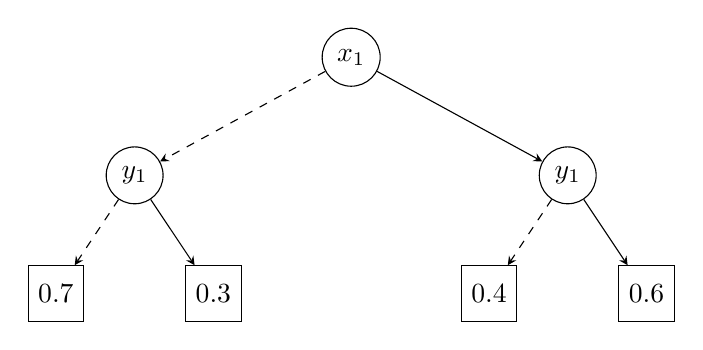
\begin{tikzpicture}[
level 1/.style={sibling distance=55mm},
level 2/.style={sibling distance=20mm},
level 3/.style={sibling distance=15mm},
level 4/.style={sibling distance=7mm}
]
\node[c] {$x_1$}
    child{ node[c]  {$y_1$} edge from parent[zeroarrow]
            child{ node[t] {0.7} 
            }
            child{ node [t] {0.3} edge from parent[onearrow]
            }
    }
    child{ node[c] {$y_1$} edge from parent[onearrow]
        child{ node[t] {0.4} edge from parent[zeroarrow]
        }
        child{ node[t] {0.6} edge from parent[onearrow]}
    }
;
    \end{tikzpicture}
    \caption{B-matrix representation in ADD}
\end{figure}

\begin{figure}
    \centering
    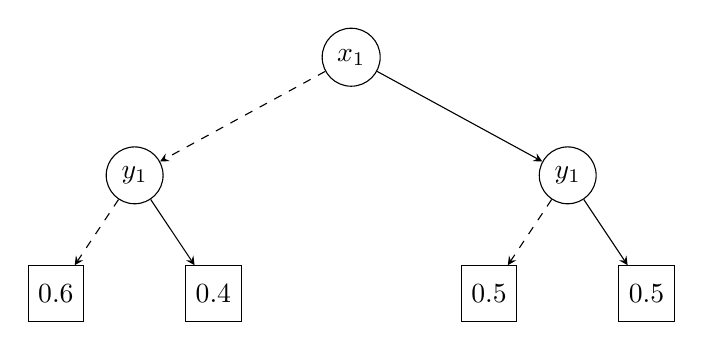
\begin{tikzpicture}[
level 1/.style={sibling distance=55mm},
level 2/.style={sibling distance=20mm},
level 3/.style={sibling distance=15mm},
level 4/.style={sibling distance=7mm}
]
\node[c] {$x_1$}
    child{ node[c]  {$y_1$} edge from parent[zeroarrow]
            child{ node[t] {0.6} 
            }
            child{ node [t] {0.4} edge from parent[onearrow]
            }
    }
    child{ node[c] {$y_1$} edge from parent[onearrow]
        child{ node[t] {0.5} edge from parent[zeroarrow]
        }
        child{ node[t] {0.5} edge from parent[onearrow]}
    }
;
    \end{tikzpicture}
    \caption{A-matrix representation in ADD}
\end{figure}

\begin{figure}
    \centering
    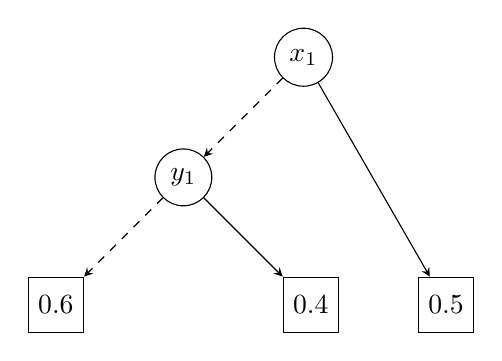
\begin{tikzpicture}[node distance=1cm and 1cm]
        \node[c] (a) {$x_1$};
        \node[c] (b) [below left=of a] {$y_1$};
        \node[t] (final-1) [below left=of b] {0.6};
        \node[t] (final-2) [below right=of b] {0.4};
        \node[t] (final-3) [right=of final-2] {0.5};

        \draw[zeroarrow] (a) -- (b);
        \draw[zeroarrow] (b) -- (final-1);
        \draw[onearrow] (b) -- (final-2);
        \draw[onearrow] (a) -- (final-3);
        
    \end{tikzpicture}
    \caption{A-matrix representation in ADD caption reduced}
\end{figure}

\begin{figure}
    \centering
    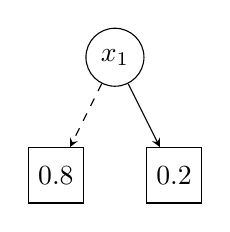
\begin{tikzpicture}
    \node[c] {$x_1$}
            child{ node[t] {0.8} edge from parent[zeroarrow] 
            }
            child{ node [t] {0.2} edge from parent[onearrow]
            }
            ;
    \end{tikzpicture}
    \caption{$\pi$-matrix representation in ADD}
\end{figure}

We can now use the ADD representation to calculate $\alpha$ and $\beta$.

When using ADD's it is important to remember, if we need to take a row from a matrix, we fix the input to the ADD by setting the x-variables to the desired row. An example is taking the third row of a matrix with 8 rows, we set, $x_1 = 1, x_2 = 1, x_3 = 0$ and $x_4 = 0$. if we need to take the second column, we set $y_1 = 1, y_2 = 0$ and $y_3 = 0, y_4 = 0$.
Hadamard product is row-wise multiplication of the matrices. So to calculate the Hadamard product of two matrices, we set the x-variables to the same row in both matrices and multiply the corresponding nodes in the ADDs.
To calculate a Hadamard product in ADD, we multiply the corresponding nodes in the ADDs, as shown in the following figure.
\begin{figure}
    \centering
    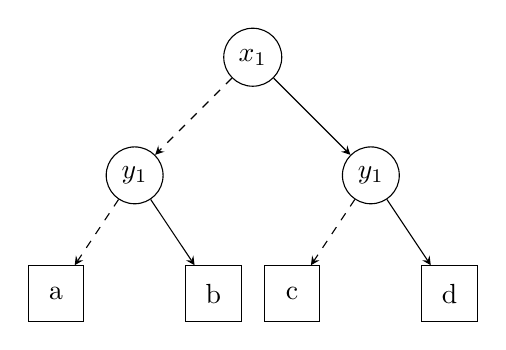
\begin{tikzpicture}[level 1/.style={sibling distance=30mm},
        level 2/.style={sibling distance=20mm},
        level 3/.style={sibling distance=15mm},
        level 4/.style={sibling distance=7mm}]
        \node[c] {$x_1$}
        child{ node[c]  {$y_1$} edge from parent[zeroarrow]
                child{ node[t] {a} 
                }
                child{ node [t] {b} edge from parent[onearrow]
                }
        }
        child{ node[c] {$y_1$} edge from parent[onearrow]
            child{ node[t] {c} edge from parent[zeroarrow]
            }
            child{ node[t] {d} edge from parent[onearrow]}
        }
    ;
    \end{tikzpicture}
    \caption{Matrix A in ADD}
\end{figure}

\begin{figure}
    \centering
    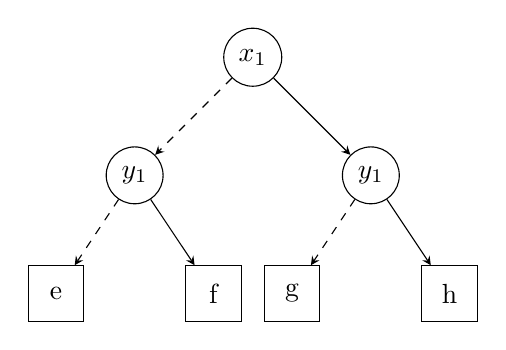
\begin{tikzpicture}[level 1/.style={sibling distance=30mm},
        level 2/.style={sibling distance=20mm},
        level 3/.style={sibling distance=15mm},
        level 4/.style={sibling distance=7mm}]
        \node[c] {$x_1$}
        child{ node[c]  {$y_1$} edge from parent[zeroarrow]
                child{ node[t] {e} 
                }
                child{ node [t] {f} edge from parent[onearrow]
                }
        }
        child{ node[c] {$y_1$} edge from parent[onearrow]
            child{ node[t] {g} edge from parent[zeroarrow]
            }
            child{ node[t] {h} edge from parent[onearrow]}
        }
    ;
    \end{tikzpicture}
    \caption{Matrix B in ADD}
\end{figure}

\begin{figure}
    \centering
    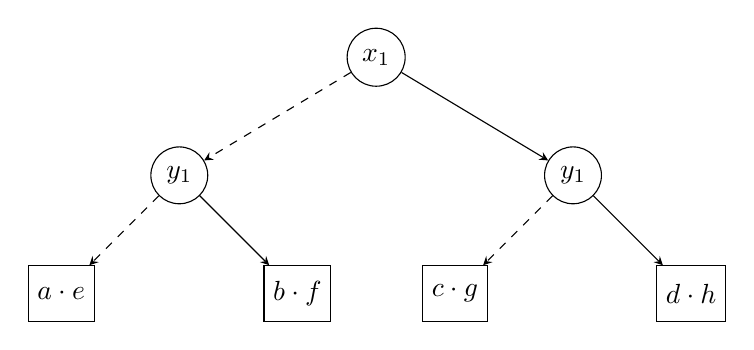
\begin{tikzpicture}[level 1/.style={sibling distance=50mm},
        level 2/.style={sibling distance=30mm},
        level 3/.style={sibling distance=40mm},
        level 4/.style={sibling distance=20mm}]
        \node[c] {$x_1$}
        child{ node[c]  {$y_1$} edge from parent[zeroarrow]
                child{ node[t] {$a \cdot e$} 
                }
                child{ node [t] {$b \cdot f$} edge from parent[onearrow]
                }
        }
        child{ node[c] {$y_1$} edge from parent[onearrow]
            child{ node[t] {$c \cdot g$} edge from parent[zeroarrow]
            }
            child{ node[t] {$d \cdot h$} edge from parent[onearrow]}
        }
    ;
    \end{tikzpicture}
    \caption{Hadamard product of A and B in ADD}
\end{figure}


Matrix multiplication is done by fixing the input to the first matrix and the output to the second matrix. We then sum the result of the Hadamard product of the rows of the first matrix and the columns of the second matrix. This is shown in the following figure.

\begin{figure}
    \centering
    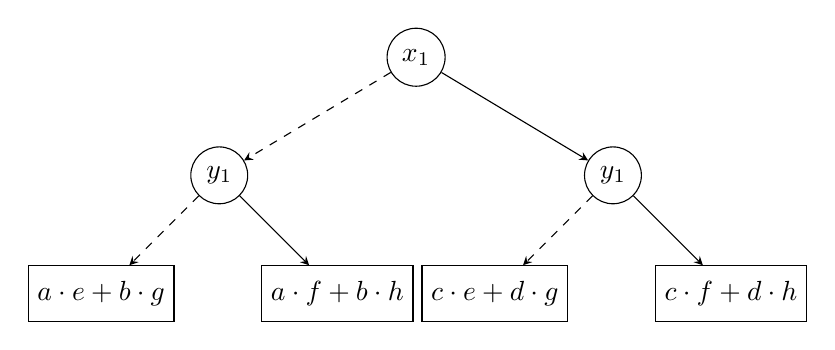
\begin{tikzpicture}[level 1/.style={sibling distance=50mm},
        level 2/.style={sibling distance=30mm},
        level 3/.style={sibling distance=40mm},
        level 4/.style={sibling distance=20mm}]
        \node[c] {$x_1$}
        child{ node[c]  {$y_1$} edge from parent[zeroarrow]
                child{ node[t] {$a \cdot e + b \cdot g$} 
                }
                child{ node [t] {$a \cdot f + b \cdot h$} edge from parent[onearrow]
                }
        }
        child{ node[c] {$y_1$} edge from parent[onearrow]
            child{ node[t] {$c \cdot e + d \cdot g$} edge from parent[zeroarrow]
            }
            child{ node[t] {$c \cdot f + d \cdot h$} edge from parent[onearrow]}
        }
    ;
    \end{tikzpicture}
    \caption{Matrix multiplication of A and B in ADD}
\end{figure}

\begin{figure}
    \centering
    \begin{tikzpicture}[level 1/.style={sibling distance=50mm},
        level 2/.style={sibling distance=30mm},
        level 3/.style={sibling distance=40mm},
        level 4/.style={sibling distance=20mm}]
        \node[c] {$x_1$}
        child{ node[c]  {$y_1$} edge from parent[zeroarrow]
                child{ node[t] {$\lambda \cdot a$} 
                }
                child{ node [t] {$\lambda \cdot b$} edge from parent[onearrow]
                }
        }
        child{ node[c] {$y_1$} edge from parent[onearrow]
            child{ node[t] {$\lambda \cdot c$} edge from parent[zeroarrow]
            }
            child{ node[t] {$\lambda \cdot d$} edge from parent[onearrow]}
        }
    ;
    \end{tikzpicture}
    \caption{Scalar product in ADD}
\end{figure}

\begin{figure*}
    \centering
    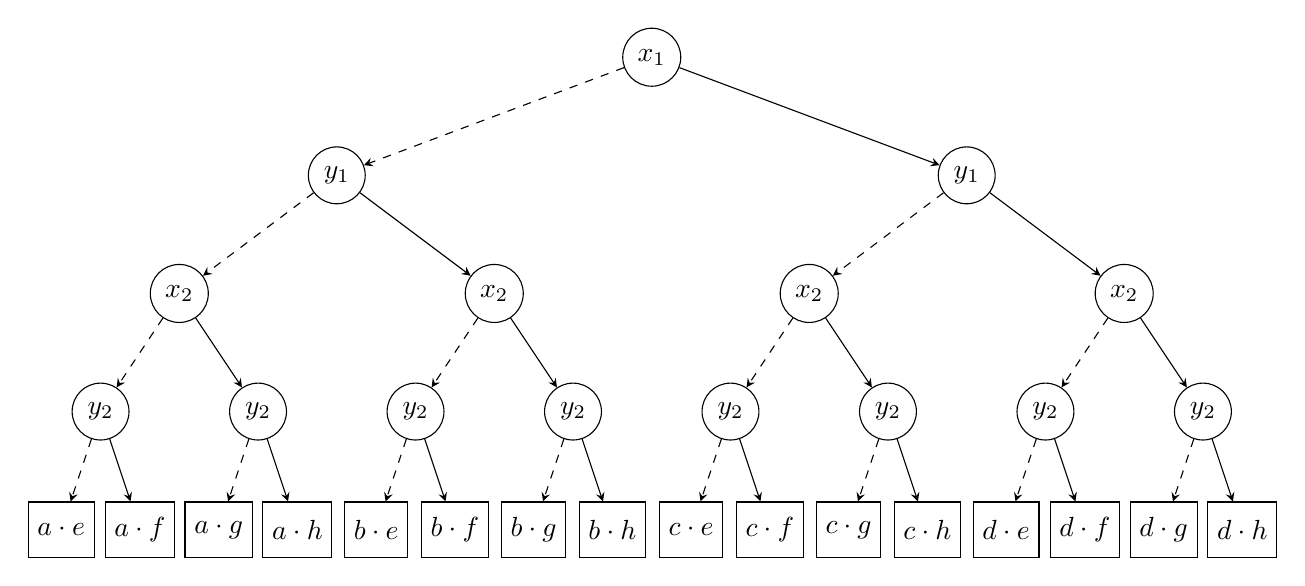
\begin{tikzpicture}[
        level 1/.style={sibling distance=80mm},
        level 2/.style={sibling distance=40mm},
        level 3/.style={sibling distance=20mm},
        level 4/.style={sibling distance=10mm}
        ]
    \node[c] {$x_1$}
        child{ node[c]  {$y_1$} edge from parent[zeroarrow]
                child{ node[c] {$x_2$} 
                        child{ node[c] {$y_2$} 
                            child{ node[t] {$a \cdot e$}}
                            child{ node[t] {$a \cdot f$} edge from parent[onearrow]} 
                        }
                        child{ node[c] {$y_2$} edge from parent[onearrow]
                            child{ node[t] {$a \cdot g$} edge from parent[zeroarrow]}
                            child{ node[t] {$a \cdot h$}} 
                        }
                }
                child{ node [c] {$x_2$} edge from parent[onearrow]
                        child{ node[c] {$y_2$}  edge from parent[zeroarrow]
                            child{ node[t] {$b \cdot e$}} 
                            child{ node[t] {$b \cdot f$} edge from parent[onearrow]} 
                        }
                        child{ node[c] {$y_2$} edge from parent[onearrow]
                            child{ node[t] {$b \cdot g$} edge from parent[zeroarrow]} 
                            child{ node[t] {$b \cdot h$}} 
                        }
                }
        }
        child{ node[c] {$y_1$} edge from parent[onearrow]
                child{ node [c] {$x_2$} edge from parent[zeroarrow]
                        child{ node[c] {$y_2$} 
                            child{ node[t] {$c \cdot e$}} 
                            child{ node[t] {$c \cdot f$} edge from parent[onearrow]} 
                        }
                        child{ node[c] {$y_2$} edge from parent[onearrow]
                            child{ node[t] {$c \cdot g$} edge from parent[zeroarrow]} 
                            child{ node[t] {$c \cdot h$}}  
                        }
                }
                child{ node [c] {$x_2$} edge from parent[onearrow]
                        child{ node[c] {$y_2$} edge from parent[zeroarrow]
                            child{ node[t] {$d \cdot e$}} 
                            child{ node[t] {$d \cdot f$} edge from parent[onearrow]} 
                        }
                        child{ node[c] {$y_2$} edge from parent[onearrow]
                            child{ node[t] {$d \cdot g$} edge from parent[zeroarrow]} 
                            child{ node[t] {$d \cdot h$}} 
                        }
                }
        }
    ;
    \end{tikzpicture}        
    \caption{Kroneker product in ADD}
\end{figure*}

\begin{figure}
    \centering
    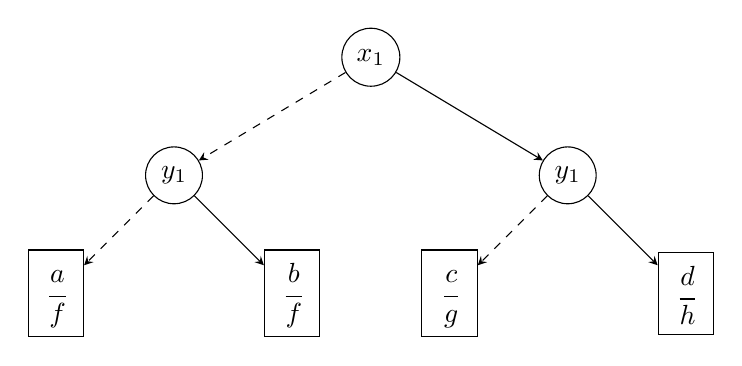
\begin{tikzpicture}[level 1/.style={sibling distance=50mm},
        level 2/.style={sibling distance=30mm},
        level 3/.style={sibling distance=40mm},
        level 4/.style={sibling distance=20mm}]
        \node[c] {$x_1$}
        child{ node[c]  {$y_1$} edge from parent[zeroarrow]
                child{ node[t] {$\cfrac{a}{f}$} 
                }
                child{ node [t] {$\cfrac{b}{f}$} edge from parent[onearrow]
                }
        }
        child{ node[c] {$y_1$} edge from parent[onearrow]
            child{ node[t] {$\cfrac{c}{g}$} edge from parent[zeroarrow]
            }
            child{ node[t] {$\cfrac{d}{h}$} edge from parent[onearrow]}
        }
    ;
    \end{tikzpicture}
    \caption{Hadamard division of A and B in ADD}
\end{figure}

\begin{figure*}
    \centering
    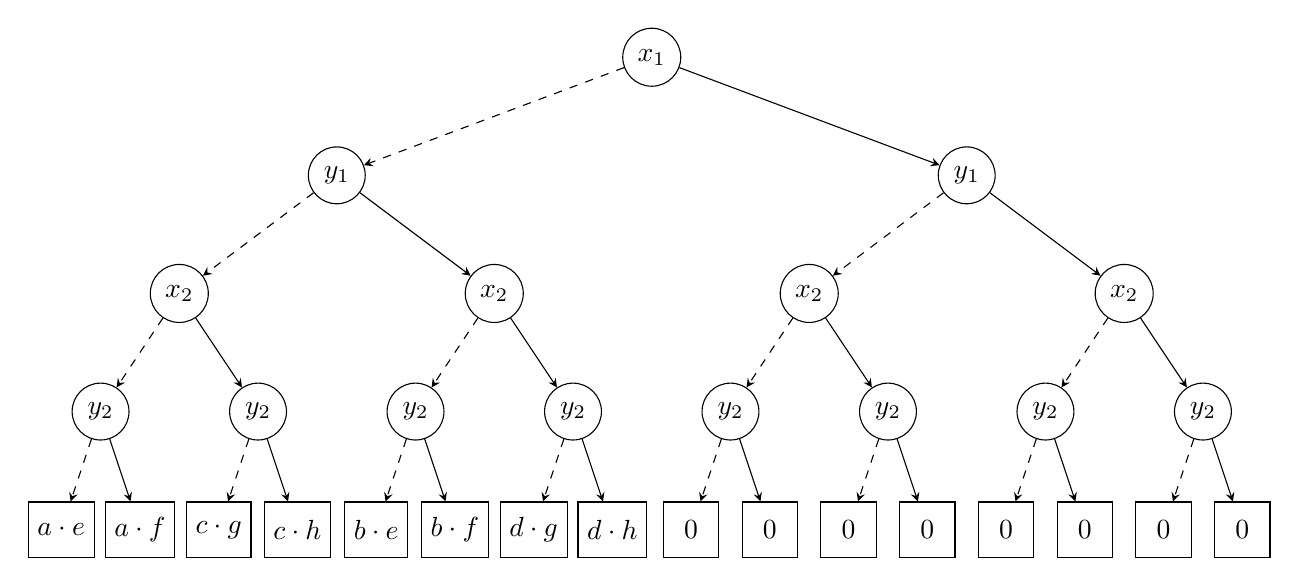
\begin{tikzpicture}[
        level 1/.style={sibling distance=80mm},
        level 2/.style={sibling distance=40mm},
        level 3/.style={sibling distance=20mm},
        level 4/.style={sibling distance=10mm}
        ]
    \node[c] {$x_1$}
        child{ node[c]  {$y_1$} edge from parent[zeroarrow]
                child{ node[c] {$x_2$} 
                        child{ node[c] {$y_2$} 
                            child{ node[t] {$a \cdot e$}}
                            child{ node[t] {$a \cdot f$} edge from parent[onearrow]} 
                        }
                        child{ node[c] {$y_2$} edge from parent[onearrow]
                            child{ node[t] {$c \cdot g$} edge from parent[zeroarrow]}
                            child{ node[t] {$c \cdot h$}} 
                        }
                }
                child{ node [c] {$x_2$} edge from parent[onearrow]
                        child{ node[c] {$y_2$}  edge from parent[zeroarrow]
                            child{ node[t] {$b \cdot e$}} 
                            child{ node[t] {$b \cdot f$} edge from parent[onearrow]} 
                        }
                        child{ node[c] {$y_2$} edge from parent[onearrow]
                            child{ node[t] {$d \cdot g$} edge from parent[zeroarrow]} 
                            child{ node[t] {$d \cdot h$}} 
                        }
                }
        }
        child{ node[c] {$y_1$} edge from parent[onearrow]
                child{ node [c] {$x_2$} edge from parent[zeroarrow]
                        child{ node[c] {$y_2$} 
                            child{ node[t] {0}} 
                            child{ node[t] {0} edge from parent[onearrow]} 
                        }
                        child{ node[c] {$y_2$} edge from parent[onearrow]
                            child{ node[t] {0} edge from parent[zeroarrow]} 
                            child{ node[t] {0}}  
                        }
                }
                child{ node [c] {$x_2$} edge from parent[onearrow]
                        child{ node[c] {$y_2$} edge from parent[zeroarrow]
                            child{ node[t] {0}} 
                            child{ node[t] {0} edge from parent[onearrow]} 
                        }
                        child{ node[c] {$y_2$} edge from parent[onearrow]
                            child{ node[t] {0} edge from parent[zeroarrow]} 
                            child{ node[t] {0}} 
                        }
                }
        }
    ;
    \end{tikzpicture}        
    \caption{Katri-Rao in ADD}
\end{figure*}

\begin{figure}
    \centering
    \begin{tikzpicture}[level 1/.style={sibling distance=50mm},
        level 2/.style={sibling distance=30mm},
        level 3/.style={sibling distance=40mm},
        level 4/.style={sibling distance=20mm}]
        \node[c] {$y_1$}
        child{ node[c]  {$x_1$} edge from parent[zeroarrow]
                child{ node[t] {a} 
                }
                child{ node [t] {c} edge from parent[onearrow]
                }
        }
        child{ node[c] {$y_1$} edge from parent[onearrow]
            child{ node[t] {b} edge from parent[zeroarrow]
            }
            child{ node[t] {d} edge from parent[onearrow]}
        }
    ;
    \end{tikzpicture}
    \caption{transpose in ADD}
\end{figure}

%To calculate $\alpha_1$ we can use the following formula:
%\[
%\alpha_1 = \pi \circ B_{y1}
%\]
%We can now calculate $\alpha_1$:
%\[
%\alpha_1 = \pi_{ADD}(0) \cdot B_{y1}(0) + \pi_{ADD}(1) \cdot B_{y1}(1) = 0.8 \cdot 0.7 + 0.2 \cdot 0.4 = 0.56
%\]
%\begin{figure}
%    \centering
%    \begin{tikzpicture}[ node distance=1cm and 1cm]
%        \node[c] (a) {$x_1$};
%        \node[t] (final-1) [below left=of a] {0.56};
%        \node[t] (final-2) [below right=of a] {0.08};
%
%        \draw[zeroarrow] (a) -- (final-1);
%        \draw[onearrow] (a) -- (final-2);
%    \end{tikzpicture}
%    \caption{$\alpha_1$-matrix representation in ADD}
%\end{figure}

%\begin{figure}
%    \centering
%    \begin{tikzpicture}[ node distance=1cm and 1cm]
%        \node[c] (a) {$x_1$};
%        \node[t] (final-1) [below left=of a] {0.1128};
%        \node[t] (final-2) [below right=of a] {0.1584};
%
%        \draw[zeroarrow] (a) -- (final-1);
%        \draw[onearrow] (a) -- (final-2);
%    \end{tikzpicture}
%    \caption{$\alpha_2$-matrix representation in ADD}
%\end{figure}

%\begin{figure}
%    \centering
%    \begin{tikzpicture}[ node distance=1cm and 1cm]
%        \node[c] (a) {$x_1$};
%        \node[t] (final-1) [below left=of a] {0.102816};
%        \node[t] (final-2) [below right=of a] {0.049728};
%
%        \draw[zeroarrow] (a) -- (final-1);
%        \draw[onearrow] (a) -- (final-2);
%    \end{tikzpicture}
%    \caption{$\alpha_3$-matrix representation in ADD}
%\end{figure}

%\begin{figure}
%    \centering
%    \begin{tikzpicture}[ node distance=1cm and 1cm]
%        \node[c] (a) {$x_1$};
%        \node[t] (final-1) [below left=of a] {0.2364};
%        \node[t] (final-2) [below right=of a] {0.252};
%
%        \draw[zeroarrow] (a) -- (final-1);
%        \draw[onearrow] (a) -- (final-2);
%    \end{tikzpicture}
%    \caption{$\beta_1$-matrix representation in ADD}
%\end{figure}

%\begin{figure}
%    \centering
%    \begin{tikzpicture}[ node distance=1cm and 1cm]
%        \node[c] (a) {$x_1$};
%        \node[t] (final-1) [below left=of a] {0.58};
%        \node[t] (final-2) [below right=of a] {0.55};
%
%        \draw[zeroarrow] (a) -- (final-1);
%        \draw[onearrow] (a) -- (final-2);
%    \end{tikzpicture}
%    \caption{$\beta_2$-matrix representation in ADD}
%\end{figure}

%\begin{figure}
%    \centering
%    \begin{tikzpicture}[ node distance=1cm and 1cm]
%        \node[c] (a) {$x_1$};
%        \node[t] (final-1) [below left=of a] {1};
%        \node[t] (final-2) [below right=of a] {1};
%
%        \draw[zeroarrow] (a) -- (final-1);
%        \draw[onearrow] (a) -- (final-2);
%    \end{tikzpicture}
%    \caption{$\beta_3$-matrix representation in ADD}
%\end{figure}

    \section{Class Diagram}\label{sec:class-diagram}
The class diagram in Figure~\ref{fig:class-diagram} shows the relationships between the different classes in the system.
The \texttt{Model} class represents the underlying model of the system, which can be a CTMC, DTMC, HMM and MDP.
The \texttt{Model} class has a aggregation relationship with the \texttt{Algorithm} class, which represents the functions used in the Baum-Welch algorithm, with and without ussing log-semiring.
The \texttt{Algorithm} class has a dependency relationship with the \texttt{CUDD} class, which is a wrapper for the CUDD library.
The \texttt{CUDD} class is used to perform the matrix operations as ADD's required by the Baum-Welch algorithm.
The \texttt{Model} class also has a aggregation relationship with the \texttt{CUDD} class, as the \texttt{Model} class uses the \texttt{CUDD} class to perform the ADD operations.

\subsection{\texttt{Model} Class}
The \texttt{Model} class serves as the foundation for representing various probabilistic models like CTMC, MDP, and DTMC. 
It holds fields needed to describe these models, such as the transition matrices, emission probabilities, and initial states, all represented using Algebraic Decision Diagrams (ADDs). 
The \texttt{Model} class also provides methods for training models, such as the Baum-Welch algorithm.

\textbf{Attributes:}
\begin{itemize}
    \item \texttt{Type\_model}: Defines the type of model (e.g., CTMC, MDP, DTMC).
    \item \texttt{transfer}: A list of ADD structures representing state transition probabilities.
    \item \texttt{Emission}: An ADD for the emission probabilities (relevant in Hidden Markov Models).
    \item \texttt{pi}: The initial state distribution, also stored as an ADD.
    \item \texttt{training\_set}: A collection of observed data.
\end{itemize}
\textbf{Methods:}
\begin{itemize}
    \item \texttt{Instantiate\_with\_parameters(prismfile, parameters: Dictionary)}: Instantiates a model with specified parameters.
    \item \texttt{Instantiate\_without\_parameters(prismfile)}: Creates a model without additional parameters.
    \item \texttt{Baum-welsh(log, Model)}: This method implements the Baum-Welch algorithm for training Hidden Markov Models, utilizing various operations from the \texttt{Algorithm} class.
\end{itemize}

\subsection{\texttt{CUDD} Class}
The \texttt{CUDD} class (CUDD Manager) is responsible for managing ADDs. These ADDs are crucial in representing the probabilistic data structures used in the \texttt{Model} class. \texttt{CUDD} provides a set of operations that allow mathematical and logical manipulation of these diagrams.

\textbf{Attributes:}
\begin{itemize}
    \item \texttt{rowvars, colvars}: Representing variables used in the ADD structures.
    \item \texttt{ADD}: The main data structure for storing probabilities or logical expressions.
    \item \texttt{Manager}: A control structure that coordinates operations on ADDs.
\end{itemize}
\textbf{Methods:}
\begin{itemize}
    \item \texttt{Hadamard(), Log\_Hadamard()}: Perform element-wise operations on ADDs.
    \item \texttt{Matrix\_mul(), Log\_matrix\_mul()}: For matrix multiplications.
    \item \texttt{Sum(), Transpose()}: Additional helper methods for summing and transposing ADDs.
\end{itemize}

\subsection{\texttt{Algorithm} Class}
The \texttt{Algorithm} class encapsulates various methods for performing probabilistic calculations. These methods are mainly used for inference in models such as Hidden Markov Models (HMM) and Markov Chains.

\textbf{Methods:}
\begin{itemize}
    \item \texttt{calculate\_alpha(), calculate\_beta()}: Compute the forward (alpha) and backward (beta) probabilities, respectively.
    \item \texttt{calculate\_gamma(), calculate\_xi()}: Intermediate probability calculations needed for parameter estimation and model training.
\end{itemize}
Each method operates on the ADD structures created and managed by the \texttt{CUDD} class, ensuring efficient computation of the probabilities.

\subsection{Relationships Between Classes}
\subsubsection{\texttt{Model} to \texttt{Algorithm}: Association Relationship}
The \texttt{Model} class uses the \texttt{Algorithm} class to compute the forward-backward probabilities and other values necessary for inference. 
The Baum-welsh(log, Model) method in \texttt{Model} invokes the relevant methods from \texttt{Algorithm} (calculate\_alpha(), calculate\_beta(), etc.) during the training process of HMMs. 
These methods, while called collectively in Baum-Welch, can also be used independently to perform specific calculations.

\subsubsection{\texttt{Model} to \texttt{CUDD}: Aggregation Relationship}
The \texttt{Model} class contains several attributes (transfer, Emission, pi) that are represented as ADDs, managed by the \texttt{CUDD} class.
This relationship is best represented as an aggregation, where the \texttt{Model} holds instances of ADD but does not directly manage their internal workings.
Instead, \texttt{CUDD} provides the operations required to manipulate and operate on these diagrams, such as matrix multiplication or element-wise functions (Hadamard products).
The \texttt{Model} depends on \texttt{CUDD} for these operations, making it an integral part of the system's backend.

\subsubsection{\texttt{Algorithm} to \texttt{CUDD}: Dependency Relationship}
The \texttt{Algorithm} class depends on the \texttt{CUDD} class for all its operations on ADDs.
Every method in \texttt{Algorithm} (e.g., calculate\_alpha(), calculate\_gamma()) relies on ADD operations provided by \texttt{CUDD}, such as Matrix\_mul() and Hadamard().
This is represented by a dependency relationship, where \texttt{Algorithm} calls \texttt{CUDD}'s methods to perform its computations.

\begin{figure}
    \centering
    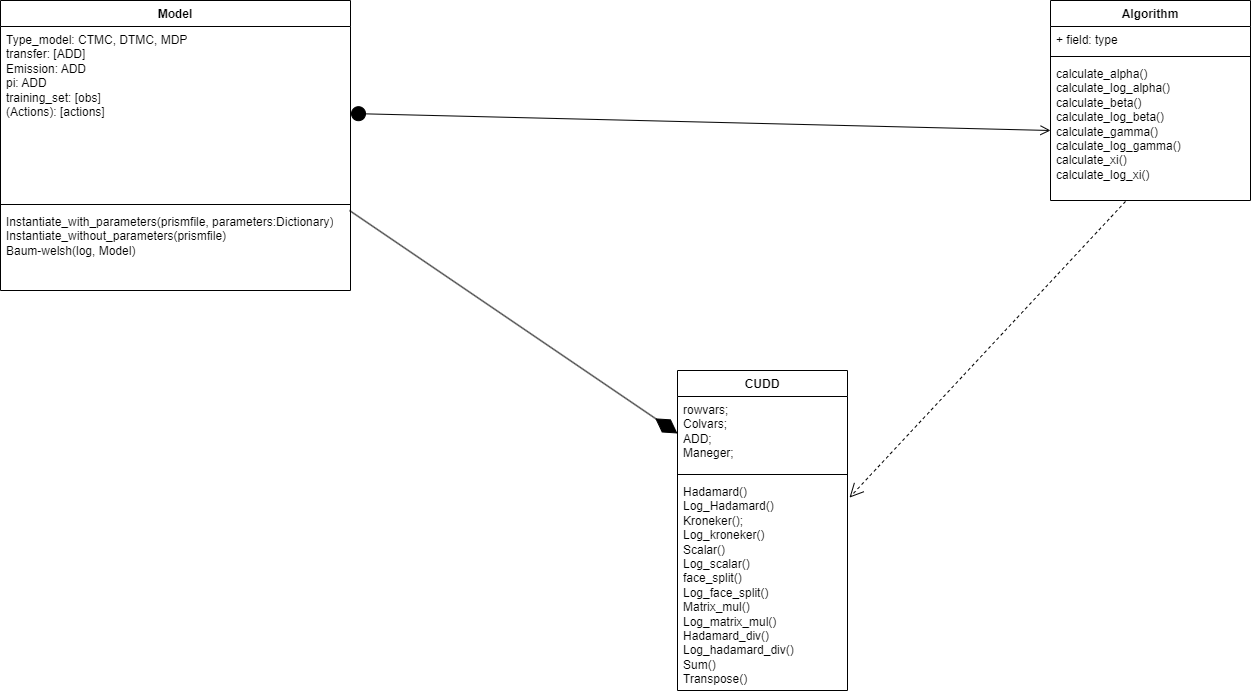
\includegraphics[width=0.5\textwidth]{figures/class-diagram.png}
    \caption{Class diagram of the system}
    \label{fig:class-diagram}
\end{figure}
    \section{Experiment}\label{sec:experiment}
%Sammenlignende Eksperimentel Evaluering af Kø- og Synkroniseringsmodeller

%Introduktion
The purpose of the experiments is to evaluate the performance of different implementations of the Baum-Welch algorithm when applied to various CTMC models. Specifically, we compare our implementation that utilize ADDs with and without the log semiring to other implementations from Jajapy, namely the original Jajapy implementation of the Baum-Welch algorithm and the improved SUDD implementation. By analyzing both parameter estimation accuracy and runtime, we aim to determine the efficiency and reliability of each implementation across multiple model types.
We also investigate the scalability of the Baum-Welch algorithm by increasing the number of states in the model and comparing the runtime of each implementation.

%Eksperimentelt Setup
We use 5 different models to test the performance of the Baum-Welch algorithm.
Each model provides a different structure and complexity level for testing the Baum-Welch algorithm. The models are derived from CTMCs and include:
\begin{itemize}
    \item \textbf{Polling}: A model representing a server polling multiple queues, often used in network communication scenarios.
    \item \textbf{Cluster}: Simulates clusters of entities competing for shared resources.
    \item \textbf{Tandem}: A series of interconnected queues where entities move sequentially from one queue to the next.
    \item \textbf{Philosophers(I) and Philosophers2(II)}: Models representing the classic synchronization problem where entities (philosophers) compete for limited resources (e.g., forks), with Philosophers2 containing one additional parameter.
\end{itemize}

In every model, we have a number of parameters we want to estimate. 
The number of parameters to estimate in each model is shown in \autoref{tab:parameters}.
The polling model is the smallest model with 2 parameters to estimate, while philosophers(II) is the largest model, with 4 parameters to estimate.'

\begin{table}[H]
    \centering
    \caption{Number of parameters to estimate in each model}
    \begin{tabular}{ll}
        \toprule
        Model & Num of parameters \\ 
        Polling & 2 \\ 
        Cluster & 3 \\ 
        Tandem & 3 \\ 
        Philosophers(I) & 3 \\ 
        Philosophers(II) & 4 \\
        \bottomrule
    \end{tabular}
    \label{tab:parameters}
\end{table}

\subsection{Parameter Estimation Accuracy}
%Beskrivelse af eksperimentet
The first experiment measures the time and accuracy of the Baum-Welch algorithm for each implementation. We generate observation sequences from each model and use the Baum-Welch algorithm to estimate the parameters of the model. We compare the estimated parameters with the true parameters of the model to evaluate the accuracy of the estimation.
%We evaluate the parameter estimation accuracy of the Baum-Welch algorithm by comparing the estimated parameters with the true parameters of the model. We use the relative formula error and relative parameter error to measure the accuracy of the estimated parameters. 

The experiment is made with the following steps:
\begin{enumerate}
    \item We load the model.
    \item Generate an observation sequence from the model with untimed steps.
    \item Calculate the model’s parameters using each variant of the Baum-Welch algorithm, recording both the parameter estimates and runtime.
    \item Repeat steps 2 and 3 ten times without changing the model, the sequence length, or whether the sequence is timed or untimed. The results are averaged to account for any variance in runtime and estimation accuracy.
    \item Repeat with timed steps to observe the effects of timing information on estimation accuracy and runtime.
    \item Compare the estimated parameters with the true parameters and record the runtime for each implementation.
    \item Move to the next model and repeat the entire process.
\end{enumerate}

Following the experiment, the estimated parameters for each implementation are compared with the true parameters for accuracy assessment. Additionally, runtime for each Baum-Welch implementation is recorded. These results are presented in tables and plots to facilitate a direct comparison of performance across models and between implementations.

Table \ref{tab:polling_results}, \ref{tab:cluster_results}, \ref{tab:tandem_results}, \ref{tab:philosophers1_results} and \ref{tab:philosophers2_results} show detailed results for each model in terms of runtime and estimation accuracy (relative formula error and relave parameter error). 



\subsection{Scalability experiment}
We also test the scalability of the Baum-Welch algorithm by increasing the number of states in a model. We use the Tandem model and increase the number of states from 28 to 1225. We then compare the runtime of the Baum-Welch algorithm for each implementation.
We run the experiment 10 times for each number of states and compare the runtime of the Baum-Welch algorithm for each implementation.

We use plots to illustrate the scalability by showing runtime across an increasing number of states for the Tandem model, highlighting each implementation's computational efficiency.

\begin{figure}
    \centering
    \includegraphics[width=0.5\textwidth]{example-image-a}
    \caption{Scalability of Baum-Welch implementations for the Tandem model}
    \label{fig:tandem_scalability}
\end{figure}

\subsection{Results}

The comparison of the Baum-Welch implementations is based on the following criteria:
\begin{itemize}
    \item \textbf{Parameter estimation accuracy}: The accuracy of the estimated parameters compared to the true parameters.
    \item \textbf{Runtime}: The time it takes to estimate the parameters.
    \item \textbf{Scalability}: How the runtime scales with the number of states in the model.
\end{itemize}

The results are displayed as tables and plots to facilitate a direct comparison of performance across models and between implementations.

\begin{table*}[]
    \centering
    \caption{Comparison of Baum-Welch implementations for Polling}
    \label{tab:polling_results}
    \begin{tabular}{llllllllll}
    \toprule
    \multirow{2}{*}{Implementation} & \multicolumn{5}{l}{Timed Observations} & \multicolumn{4}{l}{Untimed Observations} \\ \cmidrule{2-10}
    & Time(s)       & Iteration      & avg $\delta$       & avg $\phi$ & & Time(s)       & Iteration      & avg $\delta$       & avg $\phi$ \\ \cmidrule{1-1}  
    CuPAAL & 132.5 & 3.5 & 0.1 & 0.1 & & 132.5 & 3.5 & 0.1 & 0.1 \\
    CuPAAL\_log & 132.5 & 3.5 & 0.1 & 0.1 & &  132.5 & 3.5 & 0.1 & 0.1 \\
    SUDD &  23.5 & 3.5 & 0.1 & 0.1 & & 23.5 & 3.5 & 0.1 & 0.1 \\
    SUDD\_log &  0.5 & 3.5 & 0.1 & 0.1 & & 0.5 & 3.5 & 0.1 & 0.1 \\
    Jajapy &  9.5 & 3.5 & 0.1 & 0.1 & & 9.5 & 3.5 & 0.1 & 0.1 \\
    \bottomrule
    \end{tabular}
\end{table*}

\begin{table*}
    \centering
    \caption{Comparison of Baum-Welch implementations for Cluster}
    \label{tab:cluster_results}
    \begin{tabular}{llllllllll}
    \toprule
    \multirow{2}{*}{Implementation} & \multicolumn{5}{l}{Timed Observations} & \multicolumn{4}{l}{Untimed Observations} \\ \cmidrule{2-10}
    & Time(s)       & Iteration      & avg $\delta$       & avg $\phi$ & & Time(s)       & Iteration      & avg $\delta$       & avg $\phi$ \\ \cmidrule{1-1}  
    CuPAAL & 132.5 & 3.5 & 0.1 & 0.1 & & 132.5 & 3.5 & 0.1 & 0.1 \\
    CuPAAL\_log & 132.5 & 3.5 & 0.1 & 0.1 & &  132.5 & 3.5 & 0.1 & 0.1 \\
    SUDD &  23.5 & 3.5 & 0.1 & 0.1 & & 23.5 & 3.5 & 0.1 & 0.1 \\
    SUDD\_log &  0.5 & 3.5 & 0.1 & 0.1 & & 0.5 & 3.5 & 0.1 & 0.1 \\
    Jajapy &  9.5 & 3.5 & 0.1 & 0.1 & & 9.5 & 3.5 & 0.1 & 0.1 \\
    \bottomrule
    \end{tabular}
\end{table*}

\begin{table*}[]
    \centering
    \caption{Comparison of Baum-Welch implementations for Tandem}
    \label{tab:tandem_results}
    \begin{tabular}{llllllllll}
    \toprule
    \multirow{2}{*}{Implementation} & \multicolumn{5}{l}{Timed Observations} & \multicolumn{4}{l}{Untimed Observations} \\ \cmidrule{2-10}
    & Time(s)       & Iteration      & avg $\delta$       & avg $\phi$ & & Time(s)       & Iteration      & avg $\delta$       & avg $\phi$ \\ \cmidrule{1-1}  
    CuPAAL & 132.5 & 3.5 & 0.1 & 0.1 & & 132.5 & 3.5 & 0.1 & 0.1 \\
    CuPAAL\_log & 132.5 & 3.5 & 0.1 & 0.1 & &  132.5 & 3.5 & 0.1 & 0.1 \\
    SUDD &  23.5 & 3.5 & 0.1 & 0.1 & & 23.5 & 3.5 & 0.1 & 0.1 \\
    SUDD\_log &  0.5 & 3.5 & 0.1 & 0.1 & & 0.5 & 3.5 & 0.1 & 0.1 \\
    Jajapy &  9.5 & 3.5 & 0.1 & 0.1 & & 9.5 & 3.5 & 0.1 & 0.1 \\
    \bottomrule
    \end{tabular}
\end{table*}

\begin{table*}[]
    \centering
    \caption{Comparison of Baum-Welch implementations for Philosophers(I)}
    \label{tab:philosophers1_results}
    \begin{tabular}{llllllllll}
    \toprule
    \multirow{2}{*}{Implementation} & \multicolumn{5}{l}{Timed Observations} & \multicolumn{4}{l}{Untimed Observations} \\ \cmidrule{2-10}
    & Time(s)       & Iteration      & avg $\delta$       & avg $\phi$ & & Time(s)       & Iteration      & avg $\delta$       & avg $\phi$ \\ \cmidrule{1-1}  
    CuPAAL & 132.5 & 3.5 & 0.1 & 0.1 & & 132.5 & 3.5 & 0.1 & 0.1 \\
    CuPAAL\_log & 132.5 & 3.5 & 0.1 & 0.1 & &  132.5 & 3.5 & 0.1 & 0.1 \\
    SUDD &  23.5 & 3.5 & 0.1 & 0.1 & & 23.5 & 3.5 & 0.1 & 0.1 \\
    SUDD\_log &  0.5 & 3.5 & 0.1 & 0.1 & & 0.5 & 3.5 & 0.1 & 0.1 \\
    Jajapy &  9.5 & 3.5 & 0.1 & 0.1 & & 9.5 & 3.5 & 0.1 & 0.1 \\
    \bottomrule
    \end{tabular}
\end{table*}

\begin{table*}
    \centering
    \caption{Comparison of Baum-Welch implementations for Philosophers(II)}
    \label{tab:philosophers2_results}
    \begin{tabular}{llllllllll}
    \toprule
    \multirow{2}{*}{Implementation} & \multicolumn{5}{l}{Timed Observations} & \multicolumn{4}{l}{Untimed Observations} \\ \cmidrule{2-10}
    & Time(s)       & Iteration      & avg $\delta$       & avg $\phi$ & & Time(s)       & Iteration      & avg $\delta$       & avg $\phi$ \\ \cmidrule{1-1}  
    CuPAAL & 132.5 & 3.5 & 0.1 & 0.1 & & 132.5 & 3.5 & 0.1 & 0.1 \\
    CuPAAL\_log & 132.5 & 3.5 & 0.1 & 0.1 & &  132.5 & 3.5 & 0.1 & 0.1 \\
    SUDD &  23.5 & 3.5 & 0.1 & 0.1 & & 23.5 & 3.5 & 0.1 & 0.1 \\
    SUDD\_log &  0.5 & 3.5 & 0.1 & 0.1 & & 0.5 & 3.5 & 0.1 & 0.1 \\
    Jajapy &  9.5 & 3.5 & 0.1 & 0.1 & & 9.5 & 3.5 & 0.1 & 0.1 \\
    \bottomrule
    \end{tabular}
\end{table*}





    
    
    
    \printglossary[type=\acronymtype]

    \printbibliography

    \appendices % You can use \appendix if you only have a single appendix
    %! Author = Runge
%! Date = 29-12-2023

\section{Compiling in draft}\label{sec:compiling-in-draft}
You can also compile the document in draft mode.
This shows todos, and increases the space between lines to make space for your supervisors feedback.


\end{document}
